% !TeX encoding = UTF-8
% !TeX program = lualatex
% !TeX spellcheck = en_US
% !TeX root = thesis.tex

% !TeX encoding = UTF-8
% !TeX program = lualatex
% !TeX spellcheck = en_US
% !TeX root = thesis.tex


%%%%%%%%%%%%%%%%%%%%%%%%%%%%%%%%%%%%%
%BASIC OPTIONS
%%%%%%%%%%%%%%%%%%%%%%%%%%%%%%%%%%%%%


\documentclass[
%draft,
12pt,
%oneside,
twoside,
paper=a4,									% Seitengröße%
DIV=9,										% Satzspiegel: z.B. calc oder 6-15 //war ursprünglich 13
BCOR=4mm, 									% Bindekorrektur
%listof=chapterentry,						% Im Abbildungsverzeichnis und Tabellenverzeichnis auch Kapitel anzeigen
toc=bibliography,							% Literaturverzeichnis mit ins Inhaltsverzeichnis eintragen
toc=listof,
footnotes=multiple,							% mehrere Fußnoten separieren
%parindent,									% Absatzstil hier: Einrückung;
parskip=half,								% Absatzstil hier: keine Einrückung;
numbers=noenddot,							% Keine Punkte nach Nummerierung
]{scrbook}


%%%%%%%%%%%%%%%%%%%%%%%%%%%%%%%%%%%%%
%TITLEPAGE
%%%%%%%%%%%%%%%%%%%%%%%%%%%%%%%%%%%%%
%%%%%%%%%%%%%%%%%%%%%%%%%%%%%%%%%%%%%
%TITLEPAGE
%%%%%%%%%%%%%%%%%%%%%%%%%%%%%%%%%%%%%

\newcommand{\titel}{Customizing OpenFOAM to assess\\ wind-induced natural ventilation\\ potential of classrooms\newline {\Large A case study for BRAC University}}
\newcommand{\untertitel}{}
\newcommand{\HRule}{\rule{\linewidth}{0.5mm}} % New command to make the lines in the title page
\newcommand{\art}{Master's Thesis}
\newcommand{\fachgebiet}{}
\newcommand{\autor}{Patrick Kastner}
\newcommand{\wohnort}{81369 München}
\newcommand{\univname}{Technische Universität München}
\newcommand{\studienbereich}{Energy-efficient and Sustainable Building}
\newcommand{\groupname}{}
\newcommand{\deptname}{}
\newcommand{\degreename}{Master of Science (MSc)}
\newcommand{\matrikelnr}{03650879}
\newcommand{\erstgutachter}{Prof. Dipl.-Ing. Thomas Auer}
\newcommand{\zweitgutachter}{Dr. rer. nat. Wolfgang Kessling}
\newcommand{\drittgutachter}{Markus Krauß, M.Eng.}
\newcommand{\viertgutachter}{Dipl.-Ing. Christian Oberdorf}
\newcommand{\ort}{München}

%%%%%%%%%%%%%%%%%%%%%%%%%%%%%%%%%%%%%
%CUSTOM COMMANDS
%%%%%%%%%%%%%%%%%%%%%%%%%%%%%%%%%%%%%

\newcommand{\up}[2]{#1\textsuperscript{#2}}    % z.B. \up I{fdfgdfs}
\newcommand{\down}[2]{#1\textsubscript{#2}}

\newcommand{\OF}{\mbox{OpenFOAM}}
\newcommand{\CR}{\gls{CR}}
\newcommand{\WT}{\gls{WT}}
\newcommand{\BC}{\gls{BC}}
\newcommand{\ABL}{\gls{ABL}}
\newcommand{\NVP}{\gls{NVP}}
\newcommand{\USED}{{\color{red}{USED}}}
\newcommand{\BRAC}{BRAC University}
\newcommand{\CFD}{\gls{CFD}}
\newcommand{\ACR}{\gls{ACR}}
\newcommand{\kEps}{$k-\varepsilon$}
\newcommand{\kOmega}{$k-\omega$}
\newcommand{\R}{\gls{R}}
\newcommand{\COtwo}{CO$_2$}
\newcommand{\yplus}{\gls{symb:yplus}}
\newcommand{\yPlus}{\gls{symb:yplus}}
\newcommand{\SD}{\gls{SD}}


%%%%%%%%%%%%%%%%%%%%%%%%%%%%%%%%%%%%%
%FONTS
%%%%%%%%%%%%%%%%%%%%%%%%%%%%%%%%%%%%%

\usepackage{textcomp}
\usepackage[]{euler}
\usepackage{fontspec}
\usepackage{luatextra}
\usepackage{csquotes}

%FONT Combination 1

\setmainfont{Erewhon}[
Extension=.otf,
UprightFont=*-Regular,
ItalicFont=*-Italic,
BoldFont=*-Bold,
BoldItalicFont=*-BoldItalic,
SlantedFont=*-RegularSlanted,
BoldSlantedFont=*-BoldSlanted,
]
\setsansfont{texgyreheros}[
Scale=MatchLowercase,% or MatchUppercase
Extension=.otf,
UprightFont=*-regular,
ItalicFont=*-italic,
BoldFont=*-bold,
BoldItalicFont=*-bolditalic,
]

%FONT Combination 2
\setmainfont{XCharter-Roman}
\setsansfont{texgyreheros}[
Scale=MatchLowercase,% or MatchUppercase
Extension=.otf,
UprightFont=*-regular,
ItalicFont=*-italic,
BoldFont=*-bold,
BoldItalicFont=*-bolditalic,
]

%FONT Combination 3 (Adobe Fonts)

%\setmainfont{MinionPro-Regular.otf}[
%ExternalLocation=./fonts/,
%Path=fonts/,
%Ligatures=TeX,
%Numbers=OldStyle,
%SlantedFont = MinionPro-Regular.otf,
%BoldFont = MinionPro-Bold.otf ]
%\setsansfont{MyriadPro-Regular.otf}[
%ExternalLocation=./fonts/,
%Path=fonts/,
%SlantedFont = MyriadPro-It.otf,
%BoldFont = MyriadPro-Bold.otf ]
%\setmonofont{CourierStd.otf}[
%ExternalLocation=./fonts/,
%Path=fonts/,]

%LEAVE THIS UNTOUCHED FOR NOW


%%%\setmathfont{XITS Math}
%%%\setmathfont[range=\mathup/{num,latin,Latin,greek,Greek}]{Minion Pro}
%%%\setmathfont[range=\mathbfup/{num,latin,Latin,greek,Greek}]{MinionPro-Bold}
%%%\setmathfont[range=\mathit/{num,latin,Latin,greek,Greek}]{MinionPro-It}
%%%\setmathfont[range=\mathbfit/{num,latin,Latin,greek,Greek}]{MinionPro-BoldIt}
%%%\setmathfont[range=\mathscr,StylisticSet={1}]{XITS Math}
%%%\setmathfont[range={"005B,"005D,"0028,"0029,"007B,"007D,"2211,"002F,"2215 } ]{Latin Modern Math} % brackets, sum, /
%%%\setmathfont[range={"002B,"002D,"003A-"003E} ]{MnSymbol} % + - < = >
%%%\setmathrm{Minion Pro}
%%%
%%%\usepackage{luaotfload,lualatex-math}


%%%%%%%%%%%%%%%%%%%%%%%%%%%%%%%%%%%%%
%FONT MISC SETTINGS
%%%%%%%%%%%%%%%%%%%%%%%%%%%%%%%%%%%%%


\RedeclareSectionCommands[ %Linebreak after paragraphs
afterskip=1sp
]{paragraph,subparagraph}
\usepackage{etex}
\reserveinserts{20}
\usepackage[english]{babel}				% Schriftsatzerweiterung
\usepackage{alphabeta} % Use greek letters as text and in PDF bookmarks
\usepackage{bm}								% Enable bold math symbols
\usepackage{microtype}%
%\usepackage{geometry}

\makeatletter
\g@addto@macro\bfseries{\boldmath} % bold math in section heading
\makeatother

\usepackage{wrapfig}					% Von Text umflossene Grafiken
\usepackage{subfig}



\usepackage{ellipsis} % Weißraum bei Ellipsen optimal
\usepackage[NewCommands]{ragged2e} % Flattersatz mit (!) Silbentrennung
\clubpenalty = 10000 % Schusterjungen und Hurenkinder vermeiden
\widowpenalty = 10000 % Schusterjungen und Hurenkinder vermeiden
\displaywidowpenalty = 10000 % Schusterjungen und Hurenkinder vermeiden


\usepackage{marvosym}						% Euro-Symbol verfügbar machen
\usepackage[official,right]{eurosym}


%%%%%%%%%%%%%%%%%%%%%%%%%%%%%%%%%%%%%
%GRAPHICS
%%%%%%%%%%%%%%%%%%%%%%%%%%%%%%%%%%%%%

\usepackage{graphicx} 					% Grafiken einbinden
\makeatletter							% Der folgende neue Befehl bindet Bilder in der Originalgrösse ein, falls sie weniger breit als die Seite sind. Sonst wird das Bild auf Seitenbreite skaliert.
\def\ScaleIfNeeded{%
	\ifdim\Gin@nat@width>\linewidth
	\linewidth
	\else
	\Gin@nat@width
	\fi
}
\makeatother


%%%%%%%%%%%%%%%%%%%%%%%%%%%%%%%%%%%%%
%COLORS
%%%%%%%%%%%%%%%%%%%%%%%%%%%%%%%%%%%%%


\usepackage[dvipsnames]{xcolor}
\definecolor{airforceblue}{rgb}{0.36, 0.54, 0.66}
\definecolor{royalblue}{rgb}{0.0, 0.14, 0.4}
\definecolor{tumblue}{RGB}{15 , 27 , 95}
\definecolor{tumblue}{RGB}{15 , 27 , 95}
\definecolor{lightblue}{RGB}{220 , 230 , 241}
\definecolor{tum_blue}{RGB}{0, 101, 189}
\definecolor{tum_white}{RGB}{255 , 255 , 255}
\definecolor{tum_black}{RGB}{0,0,0}
%Secondary
\definecolor{tum_blue2}{RGB}{0 , 82 , 147}
\definecolor{tum_blue3}{RGB}{0 , 51 , 89}
\definecolor{tum_grey1}{RGB}{088 , 088 , 090}
\definecolor{tum_grey2}{RGB}{156 , 157 , 159}
\definecolor{tum_grey3}{RGB}{217 , 218 , 219}
%Highlights
\definecolor{tum_beige}{RGB}{218 , 215 , 203}
\definecolor{tum_orange}{RGB}{227 , 114 , 34}
\definecolor{tum_green}{RGB}{162 , 173 , 0}
\definecolor{tum_lightblue}{RGB}{152 , 198 , 234}
\definecolor{tum_turquoise}{RGB}{100 , 160 , 200}
\definecolor{darkred}{rgb}{0.7, 0.11, 0.11}



%%%%%%%%%%%%%%%%%%%%%%%%%%%%%%%%%%%%%
%URLs
%%%%%%%%%%%%%%%%%%%%%%%%%%%%%%%%%%%%%


%\KOMAoptions{DIV=last}					% Anpassung des Satzspiegels an Schriften, (nur bei DIV=calc wirksam)
\PassOptionsToPackage{hyphens}{url}
%\usepackage[hyphenbreaks]{breakurl}
\usepackage[hyphens]{url}
%\urlstyle{same}
\makeatletter
\g@addto@macro{\UrlBreaks}{\UrlOrds}
\makeatother


%URL smaller
\usepackage{relsize}
\renewcommand*{\UrlFont}{\ttfamily\smaller\relax}


%%%%%%%%%%%%%%%%%%%%%%%%%%%%%%%%%%%%%
%HYPERREF
%%%%%%%%%%%%%%%%%%%%%%%%%%%%%%%%%%%%%

%\usepackage[hang, flushmargin]{footmisc}
\usepackage[breaklinks, hidelinks,hyperfootnotes=false, unicode]{hyperref} %Clickable hyperlinks everywhere
\def\UrlBigBreaks{\do\/\do-\do:}
\hypersetup{
	draft=false,
	%    bookmarks=true,
	bookmarksopen=true,
	bookmarksopenlevel=1,  %hier darf nur ne Zahl stehen, ansonsten produziert TeX nen Fehler in Zusammenhang mit 		bookmarksopen
	bookmarksdepth=4, %deprecated
	bookmarksnumbered=true,
	linktocpage=true,       %break links correctly in listoftables/figures
	unicode=true,          % non-Latin characters in Acrobat’s bookmarks
	pdftoolbar=true,        % show Acrobat’s toolbar?
	pdfmenubar=true,        % show Acrobat’s menu?
	pdffitwindow=true,     % window fit to page when opened
	pdfstartview={XYZ null null 1.00},
	%         XYZ 	left top zoom   Sets a coordinate and a zoom factor. If any one is null, the source link value is used. null null null will give the same values as the current page.   Fit   Fits the page to the window.    FitH 	top
	%    Fits the width of the page to the window.    FitV 	left     Fits the height of the page to the window.    FitR 	left bottom right top    Fits the rectangle specified by the four coordinates to the window.    FitB  Fits the page bounding box to the window.
	%    FitBH 	top  Fits the width of the page bounding box to the window.
	%    FitBV 	left  Fits the height of the page bounding box to the window.
	pdftitle = {\titel},    % title
	pdfauthor = {\autor},     % author
	pdfsubject = {\art},   % subject of the document
	pdfcreator={\autor},   % creator of the document
	pdfproducer={\autor}, % producer of the document
	pdfkeywords= {} {} {} {}, % list of keywords
	pdfnewwindow=true,      % links in new window
	pdfpagelayout={TwoColumnRight},
	colorlinks=true,       % false: boxed links; true: colored links
	linkcolor=black,          % color of internal links
	citecolor=tumblue,        % color of links to bibliography
	filecolor=black,      % color of file links
	urlcolor=tumblue,           % color of external links
	anchorcolor =black,
	linkbordercolor={blue!35!black},          % color of internal links
	citebordercolor={blue!35!black},        % color of links to bibliography
	filebordercolor={blue!35!black},      % color of file links
	urlbordercolor={blue!35!black},           % color of external links
	menucolor =red,
	runcolor =cyan,
	pdfencoding=auto,
}


\usepackage{bookmark}
\usepackage{xspace}				% Fixes usage of spaces
%\usepackage{layout}						% Layout überprüfen
\usepackage{setspace} 	% Linespacing: singelspacing, onehalfspacing, doublespacing
\usepackage[english, plain]{fancyref} %Cross-referencing
\usepackage{upgreek}
\usepackage{lscape}						% Landscpae Seiten
\usepackage{pdflscape}					% Landscape Seiten drehen
\usepackage{gensymb}					% Celsius anzeigen
\usepackage{subfig}					% mehrere Bilder pro Zeile
\usepackage{pdfpages}
\usepackage[footnote]{acronym}			% Abkürzungsverzeichnis
\usepackage{mathtools} % braces in math environment
\usepackage{epigraph}
%\usepackage{pgfplots}
%\usepackage{pgfkeys}
\usepackage{calc}
\usepackage{tikz}
\usepackage{setspace}
%\usepackage[version=3]{mhchem}			%chemische Formeln
\usepackage[%format=hang
,labelfont=bf,
%tableposition=top %no effefct with KOMA class
]{caption} %Bildunterschriften kleiner
\renewcommand\captionfont{\footnotesize\sffamily} % Bildtitel umformatieren
\usepackage[rightcaption]{sidecap}	%caption zentr./seitl.
\makeatletter
\newenvironment{sidefigure}{\SC@float[c]{figure}}{\endSC@float} %caption zentr./seitl.
\makeatother
\makeatletter
\newenvironment{sidetable}{\SC@float[c]{table}}{\endSC@float} %caption zentr./seitl.
\makeatother


%%%%%%%%%%%%%%%%%%%%%%%%%%%%%%%%%%%%%
%UNITS
%%%%%%%%%%%%%%%%%%%%%%%%%%%%%%%%%%%%%


\usepackage[
separate-uncertainty  = true,
uncertainty-separator =  {\,},
mode = text,
output-decimal-marker ={.},
multi-part-units      = single,
range-units           = single,
%range-phrase          = {--},
]{siunitx} 		%SI Einheit
\sisetup{
	%list-final-separator = { \translate{und} },
	%range-phrase = { \translate{bis} },
	%list-pair-separator = { \translate{und} },
	%exponent-product = \cdot
	%detect-all, %apply document fonts for siunitx
	%math-rm=\mathsf,
	%text-rm=\sffamily,
	%    locale                  = US,
	%input-decimal-markers   = {.},
	%output-decimal-marker   = {.},
	%input-ignore            = {,},
	%group-digits            = true,
	%group-separator         = {,},
	%group-separator         = {},
	%tight-spacing           = true,
	%input-signs             = ,
	%input-symbols           = ,
	%input-open-uncertainty  = ,
	%input-close-uncertainty = ,
	table-align-text-pre    = false,
}
%round-mode              = figures, %places
%round-precision         = 3,
%round-integer-to-decimal= false,
%zero-decimal-to-integer= false,
%add-decimal-zero = false,
%add-integer-zero = false,

%table-space-text-pre    = (,
%table-space-text-post   = ),

\usepackage{textpos}

%%%%%%%%%%%%%%%%%%%%%%%%%%%%%%%%%%%%%
%TABLES
%%%%%%%%%%%%%%%%%%%%%%%%%%%%%%%%%%%%%

\usepackage{booktabs} % Lines betwenn tables
\usepackage{longtable}					% Tables that are longer than one page
\usepackage{tablefootnote}				% Footnote in tables
\usepackage{tabularx, longtable, array} % Tabellen
\usepackage{ltablex} %advanced longtables across multiple pages
\usepackage{ltxtable}
\usepackage{floatrow}
\floatsetup[table]{capposition=top}
\usepackage{etoolbox} %Change font of tables
\usepackage{multirow} % merge rown in tables
\usepackage{color, colortbl}	%You will need the following two packages, the first to define new colors and the latter to actually color the table

% San serif table font

%\AtBeginEnvironment{tabular}{\rmfamily}

%%%%%%%%%%%%%%%%%%%%%%%%%%%%%%%%%%%%%
%TABLE WITH SMALL FONT
%%%%%%%%%%%%%%%%%%%%%%%%%%%%%%%%%%%%%


\newenvironment{tabularsmall}{%
	\fontsize{8}{12}\selectfont\tabular
}{%
	\endtabular
}


%%%%%%%%%%%%%%%%%%%%%%%%%%%%%%%%%%%%%
%CAPTIONS
%%%%%%%%%%%%%%%%%%%%%%%%%%%%%%%%%%%%%

\usepackage{caption}
%\usepackage{subcaption}
\captionsetup[subfloat]{font=sf,size=footnotesize}
\usepackage{sidecap} %captions on the side of figures


%Captions within pdfpages
\makeatletter
\newcommand*{\AM@pagecommandstar}{}
\define@key{pdfpages}{pagecommand*}{\def\AM@pagecommandstar{#1}}
\patchcmd{\AM@output}{\begingroup\AM@pagecommand\endgroup}
{\ifthenelse{\boolean{AM@firstpage}}{\begingroup\AM@pagecommandstar\endgroup}{\begingroup\AM@pagecommand\endgroup}}{}{} % Patch to use new option
\patchcmd{\AM@split@optionsii}{\equal{pagecommand}{\AM@temp}\or}
{\equal{pagecommand}{\AM@temp}\or\equal{pagecommand*}{\AM@temp}\or}{}{}
\makeatother
%Captions within pdfpages


% Kommando zum Ausbügeln des Bugs "\subfloat ohne \caption"
\makeatletter
\providecommand\phantomcaption{\caption@refstepcounter\@captype}
\makeatother


\usepackage[]{hypcap}  %Links to image directly, not to caption


%%%%%%%%%%%%%%%%%%%%%%%%%%%%%%%%%%%%%
%MISC PACKAGES
%%%%%%%%%%%%%%%%%%%%%%%%%%%%%%%%%%%%%


\usepackage{blindtext}
\usepackage{enumitem}

%Itemize indention
\setlist[itemize,1]{leftmargin=\dimexpr 26pt-.22in}
%\setitemize{noitemsep,topsep=0pt,parsep=0pt,partopsep=0pt} % Change size of itemize environments

\usepackage{listings}
\usepackage{morewrites}
%  Multiple Columns
\usepackage{multicol}
\usepackage{emptypage} %removes headers and footers on empty pages.
%% Custom commands

\usepackage{soul}

%% New itemize environment for equations

\newenvironment{equationitem}
{ \begin{itemize}
		\setlength{\itemsep}{1pt}
		\setlength{\parskip}{1pt}
		\setlength{\parsep}{1pt}}
	{ \end{itemize}     }


%% Appendix in toc

\usepackage[
%  toc
]{appendix}

\usepackage[
% obeyDraft
]{todonotes}

%% Counters for figures and tables

\usepackage[figure,table,equation]{totalcount}


\usepackage{placeins} %clear floats without new page



%%%%%%%%%%%%%%%%%%%%%%%%%%%%%%%%%%%%%
%BIBLIOGRAPHY
%%%%%%%%%%%%%%%%%%%%%%%%%%%%%%%%%%%%%

\usepackage[compress,sort,
numbers
]{natbib}					% Naturwissenschaftlicher Zitierstil
%\bibliographystyle{agsm}
\bibliographystyle{dinat}
%\bibliographystyle{newapa}
\renewcommand*{\bibfont}{\sffamily}

%% Change Bibliography Header


\makeatletter
\renewcommand\bibsection{%
	%	\chapter*{{\sffamily\huge\bibname}\@mkboth{\sffamily\MakeUppercase{\bibname}}{\sffamily\bibname}}%
	\chapter*{{\sffamily\huge\bibname}\@mkboth{\sffamily\bibname}{\sffamily\bibname}}%
}%
\makeatother




%%% APACITE

%\usepackage[%nodoi,
%nosectionbib,numberedbib]{apacite}
%\bibliographystyle{apacite}
%\AtBeginDocument{\urlstyle{APACsame}}

%\renewcommand\bibliographytypesize{\small}
%\renewcommand\bibliographystyle{apacite}



%Backlinks vom LitVerz zu den Seiten
% #1: number of distinct back references
% #2: backref list with distinct entries
% #3: number of back references including duplicates
% #4: backref list including duplicates
\RequirePackage[hyperpageref]{backref}
\renewcommand{\backreflastsep}{ and~}
\renewcommand{\backreftwosep}{ and~}
\renewcommand{\backref}[1]{}% for backref < 1.33 necessary
\renewcommand{\backrefalt}[4]{
	\ifnum#1=0
	%No cited.
	\else
	\ifnum#1=1
	\footnotesize \mbox{(cited on page #2)}
	\else
	%\footnotesize \mbox{{\color{darkred}(cited on pages #2)}}
	\footnotesize \mbox{(cited on pages #2)}
	\fi
	\fi
}


%%%%%%%%%%%%%%%%%%%%%%%%%%%%%%%%%%%%%
%GLOSSARIES
%%%%%%%%%%%%%%%%%%%%%%%%%%%%%%%%%%%%%

\usepackage[
nomain,
nonumberlist,
acronym,
%section
]
{glossaries-extra}

\glsaccessname{unit}
\setlength{\glsdescwidth}{15cm}
\glssetcategoryattribute{acronym}{glossdescfont}{textsf}
\glssetcategoryattribute{acronym}{glossnamefont}{textsf}
\setabbreviationstyle[acronym]{long-short}

\glssetnoexpandfield{unit}

\newglossarystyle{symbunitlong}{%
	\vspace*{.3cm}
	\setglossarystyle{long3col}% base this style on the list style
	\renewenvironment{theglossary}{% Change the table type --> 3 columns
		\begin{longtable}{lp{0.6\glsdescwidth}>{\arraybackslash}p{2cm}}}%
		{\end{longtable}}%
	%
	\renewcommand*{\glossaryheader}{%  Change the table header
		\sffamily\bfseries Sign & \sffamily\bfseries Description & \sffamily\bfseries Unit \\
		%\hline
		\endhead}
	\renewcommand*{\glossentry}[2]{%  Change the displayed items
		\glstarget{##1}{\sffamily\glossentryname{##1}} %
		& \sffamily\glossentrydesc{##1}% Description
		& \sffamily\glsunit{##1}  \tabularnewline
	}
}



\usepackage{smartdiagram}

%%%%%%%%%%%%%%%%%%%%%%%%%%%%%%%%%%%%%
%CUSTOMIZE TOC
%%%%%%%%%%%%%%%%%%%%%%%%%%%%%%%%%%%%%

%Differrent font in TOC
\usepackage[titles,subfigure]{tocloft} % Change font of Chapters,  LOF and LOT

\setlength{\cftbeforechapskip}{2ex}
\setlength{\cftbeforesecskip}{0.8ex}
\setlength{\cftbeforesubsecskip}{0.8ex}

\renewcommand{\cftchapfont}{%
	\sffamily\bfseries
}
\renewcommand{\cftchappagefont}{\sffamily}
\renewcommand{\cftsecfont}{\sffamily}
\renewcommand{\cftsecpagefont}{\sffamily}
\renewcommand{\cftsubsecfont}{\sffamily}
\renewcommand{\cftsubsecpagefont}{\sffamily}


\renewcommand\cftloftitlefont{\sffamily}
\renewcommand\cftfigfont{\sffamily}
\renewcommand\cftfigpagefont{\sffamily}

\renewcommand\cftlottitlefont{\sffamily}
\renewcommand\cfttabfont{\sffamily}
\renewcommand\cfttabpagefont{\sffamily}


% TOC depth
%\setcounter{secnumdepth}{4}


%%%%%%%%%%%%%%%%%%%%%%%%%%%%%%%%%%%%%
%CUSTOM PAGE LAYOUT
%%%%%%%%%%%%%%%%%%%%%%%%%%%%%%%%%%%%%

%Code for Headers and Footers adapted from http://www.kfiles.de

\newlength{\marginWidth}
\setlength\marginWidth{\marginparwidth+\marginparsep}
\newlength{\fulllinewidth}
\setlength\fulllinewidth{\textwidth+\marginWidth}

\usepackage{truncate} %Um zu lange Kapiteltitel abzuschneiden

\footskip=1.6cm
\makeatletter % = mache @ letter

%Vordefinition mehrfachverwendeter Teile
\def\oddfootSTANDARD{
	\renewcommand{\@oddfoot}{
		\hbox to\textwidth{\vbox{\hbox to\textwidth{
					\hfill
					\strut
					\hspace{1pt}
		}}}
		\hbox to\marginWidth{\vbox{\hbox to\marginWidth{
					\strut %unsichtbares Zeichen
					%               \large %Größe der Seitenzahl
					\hspace{5pt}
					\vrule width 1pt height 1cm
					\hspace{8pt}
					\textsf{\thepage}
					\hfill
		}}}\hss
	}
}

\def\evenfootSTANDARD{
	\renewcommand{\@evenfoot}{
		\hspace{-\marginWidth}
		\hbox to\marginWidth{\vbox{\hbox to\marginWidth{
					%         \large
					\strut %unsichtbares Zeichen
					\hfill
					\textsf{\thepage}
					\hspace{5pt}
					\vrule width 1pt height 1cm
					\hspace{7pt}
		}}}\hss
	}
}


%Standardstil für die gesamte Dissertation
\newcommand{\ps@thesis}{
	\renewcommand{\@oddhead}{
		\hbox to\textwidth{\vbox{\hbox to\textwidth{
					\textsf
					\hfill
					\rightmark
					\strut
					\hspace{1pt}
		}}}
		\hbox to\marginWidth{\vbox{\hbox to\marginWidth{
					\strut %unsichtbares Zeichen
					\hspace{5pt}
					\vrule width 1pt
					\hspace{5pt}
					\textsf{\thesection}  %%Zuständig für Nummerierung rechts oben; thesection produziert X.0, X.1
					\hfill
		}}}\hss
	}

	\renewcommand{\@evenhead}{
		\hspace{-\marginWidth}
		\hbox to\marginWidth{\vbox{\hbox to\marginWidth{
					\hfill
					\strut %unsichtbares Zeichen
					\textbf{\textsf{Chapter~\thechapter}}
					\hspace{5pt}
					\vrule width 1pt
					\hspace{7pt}
					\strut
		}}}\hss

		\hbox to\textwidth{\vbox{\hbox to\textwidth{
					\strut %unsichtbares Zeichen
					\truncate{.9\textwidth}{\leftmark}
					\hfill
		}}}\hss
	}

	\oddfootSTANDARD
	\evenfootSTANDARD
}


%Der PLAIN-Style der Chapter- und Sonderseiten muss redefiniert werden.
\renewcommand{\ps@plain}{
	\let\@oddhead\@empty
	\let\@evenhead\@empty
	\let\@evenfoot\@empty
	\oddfootSTANDARD
}

%Spezieller Stil für Inhaltsverzeichnis und Literaturverzeichnis (ohne Nummern wie 0.0 oder B.0)
\newcommand{\ps@thesisINTRO}{
	\renewcommand{\@oddhead}{
		\hbox to\textwidth{\vbox{\hbox to\textwidth{
					\textsf
					\hfill
					\textsf{\rightmark}
					\strut
					\hspace{1pt}
		}}}
		\hbox to\marginWidth{\vbox{\hbox to\marginWidth{
					\strut %unsichtbares Zeichen
					\hspace{5pt}
					\vrule width 1pt
					\hspace{5pt}
					\textsf{\thechapter}  %%Zuständig für Nummerierung rechts oben; thesection produziert X.0, X.1
					\hfill
		}}}\hss
	}

	\renewcommand{\@evenhead}{
		\hspace{-\marginWidth}
		\hbox to\marginWidth{\vbox{\hbox to\marginWidth{
					\hfill
					\strut %unsichtbares Zeichen
					\textbf{\textsf{Chapter}}
					\hspace{5pt}
					\vrule width 1pt
					\hspace{7pt}
					\strut
		}}}\hss

		\hbox to\textwidth{\vbox{\hbox to\textwidth{
					\strut %unsichtbares Zeichen
					\truncate{.9\textwidth}{\leftmark}
					\hfill
		}}}\hss
	}

	\oddfootSTANDARD
	\evenfootSTANDARD
}


\newcommand{\ps@thesisAPPENDIX}{
	\renewcommand{\@oddhead}{
		\hbox to\textwidth{\vbox{\hbox to\textwidth{
					\textsf
					\hfill
					\rightmark
					\strut
					\hspace{1pt}
		}}}
		\hbox to\marginWidth{\vbox{\hbox to\marginWidth{
					\strut %unsichtbares Zeichen
					\hspace{5pt}
					\vrule width 1pt
					\hspace{5pt}
					\textsf
					\thechapter %\\thesection  %%Zuständig für Nummerierung rechts oben; thesection produziert X.0, X.1
					\hfill
		}}}\hss
	}

	\renewcommand{\@evenhead}{
		\hspace{-\marginWidth}
		\hbox to\marginWidth{\vbox{\hbox to\marginWidth{
					\hfill
					\strut %unsichtbares Zeichen
					\textbf{\textsf{Appendix~\thechapter}}
					\hspace{5pt}
					\vrule width 1pt
					\hspace{7pt}
					\strut
		}}}\hss

		\hbox to\textwidth{\vbox{\hbox to\textwidth{
					\strut %unsichtbares Zeichen
					\truncate{.9\textwidth}{\leftmark}
					\hfill
		}}}\hss
	}

	\oddfootSTANDARD
	\evenfootSTANDARD
}


\newcommand{\ps@thesisLISTS}{
	\renewcommand{\@oddhead}{
		\hbox to\textwidth{\vbox{\hbox to\textwidth{
					\textsf
					\hfill
					\textsf{\rightmark}
					\strut
					\hspace{1pt}
		}}}
		\hbox to\marginWidth{\vbox{\hbox to\marginWidth{
					\strut %unsichtbares Zeichen
					\hspace{5pt}
					\vrule width 1pt
					\hspace{5pt}
					\textsf
					\thechapter  %%Zuständig für Nummerierung rechts oben; thesection produziert X.0, X.1
					\hfill
		}}}\hss
	}

	\renewcommand{\@evenhead}{
		\hspace{-\marginWidth}
		\hbox to\marginWidth{\vbox{\hbox to\marginWidth{
					\hfill
					\strut %unsichtbares Zeichen
					\textbf{\textsf{Chapter}}
					\hspace{5pt}
					\vrule width 1pt
					\hspace{7pt}
					\strut
		}}}\hss

		\hbox to\textwidth{\vbox{\hbox to\textwidth{
					\strut %unsichtbares Zeichen
					%	\truncate{.9\textwidth}{\textsf{\MakeUppercase{\leftmark}}}% Zuständig für Variable hinter |
					\truncate{.9\textwidth}{\textsf{\leftmark}}% Zuständig für Variable hinter |
					\hfill
		}}}\hss
	}

	\oddfootSTANDARD
	\evenfootSTANDARD
}




\newcommand{\ps@reallyempty}{
	\let\@oddhead\@empty
	\let\@evenhead\@empty
	\let\@oddfoot\@empty
	\let\@evenfoot\@empty
}


\renewcommand{\chaptermark}[1]{\markboth{\textsf{#1}}{}}%markboth hat zwei argumente für die linke und rechte seite
\renewcommand{\sectionmark}[1]{\markright{\textsf{#1}}}

\makeatother % = mache @ wieder zu nicht-Buchstaben
\pagestyle{thesis}



%%Problem mit den Seitenzahlen und Headern auf leeren Seiten nach Kapiteln:
\let\origdoublepage\cleardoublepage
\newcommand{\clearemptydoublepage}{%
	\clearpage
	{\pagestyle{empty}\origdoublepage}%
}
\let\cleardoublepage\clearemptydoublepage




%%%%%%%%%%%%%%%%%%%%%%%%%%%%%%%%%%%%%
%INDEX
%%%%%%%%%%%%%%%%%%%%%%%%%%%%%%%%%%%%%

\usepackage{makeidx}
\makeindex
\usepackage[totoc,columns=2,minspace=100pt]{idxlayout} %modify layout of index



%%%%%%%%%%%%%%%%%%%%%%%%%%%%%%%%%%%%%
%HELPER FOR FORMATTING GRAPHICS
%https://www.queryxchange.com/q/24_86356/how-to-trim-clip-crop-graphics-without-trial-and-error/
%%%%%%%%%%%%%%%%%%%%%%%%%%%%%%%%%%%%%


%\newcommand{\showgrid}[2]{%
%	\newcommand{\gridlen}{2}  % This determines the size of the squares that later appear: 2 = 0.4 cm % 5 = 1 cm  % 20 = 4 cm
%	\resizebox{#1}{!}{%
%		\begin{tikzpicture}[inner sep=0]
%		% Bild laden
%		\node[anchor=south west] (image) at (0, 0) {#2};
%		% Koordinaten fast oben rechts
%		\path (image.north east) -- ++(-\gridlen, -\gridlen) coordinate (obenrechts);
%
%		\begin{scope}[red]
%		% Gitter unten links
%		\draw[xstep=.2, ystep=.2, very thin] (0, 0) grid (\gridlen, \gridlen);
%		\draw[xstep=1, ystep=1, semithick] (0, 0) grid (\gridlen, \gridlen);
%		% Gitter oben rechts
%		\draw[xstep=.2, ystep=.2, shift={(obenrechts)}, very thin] (0, 0) grid (\gridlen, \gridlen);
%		\draw[xstep=1, ystep=1, shift={(obenrechts)}, semithick] (0, 0) grid (\gridlen, \gridlen);
%
%		% Rahmen
%		\draw (0, 0) rectangle (image.north east);
%		\end{scope}
%		\end{tikzpicture}%
%	}
%}

%Example:
%\showgrid{0.8\linewidth}{\includegraphics[clip, trim=31mm 58mm 102mm 31mm]{Test.pdf}}

\usepackage{tikz}

% Linen über Graphiken
\newcommand{\showgrid}[3][5]{%
	\providecommand{\griddepth}{#1}
	\resizebox{#2}{!}{%
		\begin{tikzpicture}[inner sep=0]
		% Bild laden
		\node[anchor=south west] (image) at (0, 0) {#3};
		% Linien einfügen
		\begin{scope}[red]
		% Äußere Schleife für dicke Rechtecke
		\foreach \iThick in {0, ..., \griddepth} {%
			\path (image.north east) ++(-\iThick, -\iThick) coordinate(topright);
			\draw[semithick] (\iThick, \iThick) rectangle (topright);
			% Zwischen den Linien auffüllen
			\ifnum\iThick<\griddepth
			% dünne Rechtecke
			\foreach \iThin in {1, ..., 4} {%
				\path (image.north east) ++(-\iThick, -\iThick) ++(-\iThin/5, -\iThin/5) coordinate(topright);
				\draw[very thin] (\iThick, \iThick) ++(\iThin/5, \iThin/5) rectangle (topright);
			}
			\fi
		}
		\end{scope}
		\end{tikzpicture}
	}
}

%Example:
%\showgrid[1]{0.8\linewidth{\includegraphics[clip, trim=20mm 34mm 8mm 16mm]{Test.pdf}}
%
%The thick lines have a distance of 10mm, the thin ones of 2mm. This is independent of the image if no width or height argument is passed to the image.



%%%%%%%%%%%%%%%%%%%%%%%%%%%%%%%%%%%%%
%LATEX OVERLAY GENERATOR
%%%%%%%%%%%%%%%%%%%%%%%%%%%%%%%%%%%%%

%%%%%%%%%%%%%%%%%%%%%%%%%%%%%%%%%%%%%
%LATEX OVERLAY GENERATOR
%%%%%%%%%%%%%%%%%%%%%%%%%%%%%%%%%%%%%

%%%%%%%%%%%%%%%%%%%%%%%%%%%%%%%%%%%%%%%%%%%%%%%%%%%%%%%%%%%%%%%%%%%%%%
% LaTeX Overlay Generator - Annotated Figures v0.0.1
% Created with http://ff.cx/latex-overlay-generator/
% If this generator saves you time, consider donating 5,- EUR! :-)
%%%%%%%%%%%%%%%%%%%%%%%%%%%%%%%%%%%%%%%%%%%%%%%%%%%%%%%%%%%%%%%%%%%%%%
%\annotatedFigureBoxCustom{bottom-left}{top-right}{label}{label-position}{box-color}{label-color}{border-color}{text-color}
\newcommand*\annotatedFigureBoxCustom[8]{\draw[#5,thick,rounded corners] (#1) rectangle (#2);\node at (#4) [fill=#6,thick,shape=circle,draw=#7,inner sep=2pt,font=\sffamily,text=#8] {\textbf{#3}};}
%\annotatedFigureBox{bottom-left}{top-right}{label}{label-position}
\newcommand*\annotatedFigureBox[4]{\annotatedFigureBoxCustom{#1}{#2}{#3}{#4}{white}{white}{black}{black}}
\newcommand*\annotatedFigureText[4]{\node[draw=none, anchor=south west, text=#2, inner sep=0, text width=#3\linewidth,font=\sffamily] at (#1){#4};}

\newcommand*\annotatedFigureBoxCustomBlack[8]{\draw[#5,thick,rounded corners] (#1) rectangle (#2);\node at (#4) [fill=#6,thick,shape=circle,draw=#7,inner sep=2pt,font=\sffamily,text=#8] {\textbf{#3}};}
%\annotatedFigureBox{bottom-left}{top-right}{label}{label-position}
\newcommand*\annotatedFigureBoxBlack[4]{\annotatedFigureBoxCustomBlack{#1}{#2}{#3}{#4}{black}{white}{black}{black}}
\newcommand*\annotatedFigureTextBlack[4]{\node[draw=none, anchor=south west, text=#2, inner sep=0, text width=#3\linewidth,font=\sffamily] at (#1){#4};}

\newcommand*\annotatedFigureBoxCustomGray[8]{\draw[#5,thick,rounded corners] (#1) rectangle (#2);\node at (#4) [fill=#6,thick,shape=circle,draw=#7,inner sep=2pt,font=\sffamily,text=#8] {\textbf{#3}};}
%\annotatedFigureBox{bottom-left}{top-right}{label}{label-position}
\newcommand*\annotatedFigureBoxGray[4]{\annotatedFigureBoxCustomBlack{#1}{#2}{#3}{#4}{gray}{white}{gray}{black}}
\newcommand*\annotatedFigureTextGray[4]{\node[draw=none, anchor=south west, text=#2, inner sep=0, text width=#3\linewidth,font=\sffamily] at (#1){#4};}

\newenvironment {annotatedFigure}[1]{\centering\begin{tikzpicture}
	\node[anchor=south west,inner sep=0] (image) at (0,0) { #1};\begin{scope}[x={(image.south east)},y={(image.north west)}]}{\end{scope}\end{tikzpicture}}
%%%%%%%%%%%%%%%%%%%%%%%%%%%%%%%%%%%%%%%%%%%%%%%%%%%%%%%%%%%%%%%%%%%%%% 





%%%%%%%%%%%%%%%%%%%%%%%%%%%%%%%%%%%%%
%CLEAR DOUBLE PAGE PROPERLY
%%%%%%%%%%%%%%%%%%%%%%%%%%%%%%%%%%%%%

%Input something on the left page, use \cleardoublepage to force on right
\makeatletter
\newcommand*{\cleartoleftpage}{%
	\clearpage
	\if@twoside
	\ifodd\c@page
	\hbox{}\newpage
	\if@twocolumn
	\hbox{}\newpage
	\fi
	\fi
	\fi
}
\makeatother


\usepackage[percent]{overpic}
%%%%%%%%%%%%%%%%%%%%%%%%%%%%%%%%%%%%%
%Fix warnings
%%%%%%%%%%%%%%%%%%%%%%%%%%%%%%%%%%%%%
\usepackage{silence}\WarningFilter{fixltx2e}{}

\input{glossaries}

\begin{document}

% Cover 
\includepdf[pages=1,trim=28cm 1.3cm 2.1cm 1.2cm,,fitpaper=false, pagecommand*={\thispagestyle{empty}}]{cover/cover.pdf}	
\cleardoublepage
%
\pagenumbering{roman}
%
\singlespacing
\include{title}
\include{abstract}
\include{dedication}
\include{acknowledgments}

\singlespacing

{\pagestyle{plain}
\pdfbookmark[chapter]{\contentsname}{toc}
\tableofcontents
\clearpage}

% Glossaries
\glsaddall

%% Acronyms
{\pagestyle{plain}
\printglossary[type=\acronymtype,style=long]
\clearpage}

%% Symbols 
{\pagestyle{plain}
\printglossary[type=symbolslist,style=symbunitlong]
\clearpage}
	

\cleardoublepage
\pagenumbering{arabic}

% Chapters
\include{1_chapter}
\glsresetall
% !TeX encoding = UTF-8
% !TeX program = lualatex
% !TeX spellcheck = en_US
% !TeX root = thesis.tex

\chapter{Building aerodynamics}
\label{chap:building_aerodynamics}

This chapter gives an overview on flow characteristics for bluff bodies as well as the basics of fluid dynamics necessary for understanding natural ventilation. The chapter ends with a summary of prediction models for natural ventilation, how they have evolved and which limitations should be considered.  

%
% %
% % %
% % % %
% % %
% %
%


\section{Basics of fluid dynamics}
\label{sec:basic_of_fluid_flow}


\subsection{Flow characteristics around bluff bodies}

Geometries in building aerodynamics are often simplified to cuboids. These geometries, characterized by flat surfaces and sharp corners are commonly referred to as "bluff bodies". Streamlines around those bodies do not follow their shape. Flow separation occurs at sharp edges or corners where the flow momentum exceeds weaker viscous forces. This leads to a development of shear layers as well as a  turbulent wake area behind the body (see \fref{fig:flowaroundbuilding}).


\begin{figure}[htb]
	\centering
	\includegraphics[width=0.9\linewidth, trim= 0cm 1cm 0cm 0cm, clip]{images/flow_around_building}
	\captionsetup{format=plain}%,labelsep=newline}
	\caption[Flow characteristics around a bluff body]{Horizontal section of flow characteristics around a bluff body. The Bernoulli's equation for airflow is valid for the mean flow along a streamline. Adapted from \cite{Aynsley1999}.}
	\label{fig:flowaroundbuilding}
\end{figure}





\subsection{Bernoulli equation}

The Bernoulli equation relates fluid pressure energy, kinetic energy, as well as potential energy of fluid flow along a streamline to each other. It may be considered as a measure of conservation of energy appropriate for fluid flows. Despite small pressure variations, density is considered to be constant for most flows of liquids and gases at low Mach numbers ($Ma \leq \num{0.3}$) \citep{fischer2008experimentelle, Hucho2011}. A further assumption is that the fluid is non-viscous and its flow is steady. The equation for any arbitrary point along a streamline is:

\begin{equation}
p_{tot} = p_{stat} + p_{dyn} + \rho \cdot g \cdot z = constant
\end{equation}

The total pressure refers to the sum of the aforementioned parts. If the variation in temperature is to be neglected or sufficiently small to be ignored, there is no significant change in potential energy along the streamline. Thus,  the above equation reduces to the following simplified form:

\begin{equation}
p_{tot} = p_{stat} + p_{dyn} = constant
\end{equation}

Static pressure is the pressure at a specific point in a fluid acting in all directions. Static pressure can always
be defined, whether or not the fluid is in motion.
Dynamic pressure represents kinetic energy per unit volume of a fluid particle acting in direction of the flow. It is defined as:

\begin{equation}
q = \frac{1}{2} \cdot \rho \cdot u^2
\end{equation}


This equation forms the basis of most air flow calculations used. When using the equation for a streamline around a bluff body, it is evident that the maximum pressure occurs at a point where the flow is brought to rest. This is commonly referred to as the stagnation point. Here, the kinetic energy of the approaching flow is converted into static pressure. Thus, the maximum dynamic pressure is equal to $0.5 \rho u^2$ (see \fref{fig:flowaroundbuilding}).



%The velocity then can be calculated as: 
%
%
%\begin{equation}
%u = \sqrt{ \frac{2 \cdot q}{\rho} }
%\end{equation}



A flow occurs if an opening is placed onto a wall separating two regions of air with different pressure levels.
By evaluating the discharge coefficient, the volumetric flow rate is given by:

\begin{equation}
Q  = S \cdot C_d \cdot A  \sqrt{ \dfrac{2\cdot|\Delta p|}{\rho}}
\end{equation}


where

\begin{equation}
S  = Sign [\Delta p]
\end{equation}

For a rectangular opening, the discharge coefficient $C_d$ is usually assumed to be in the range of \num{0.6} and \num{0.7} \citep{Chu2009}.

%\begin{equation}
%C_d  = \frac{\dot{m}}{A} \sqrt{\frac{\rho}{2\Delta p}}
%\end{equation}

%Rearranging the definition of $C_d$, the flow rate through the opening is given by 

For a cross-ventilation layout with two openings on opposite walls, a more advanced equation can be defined as: 

\begin{equation}
q = \frac{Q}{u_{H} A_{1}} = C_{d_1} \left[ \frac{r_{a}^2 C_{d_r}^2 }{1+ r_{a}^2 C_{d_r}^2} |c_{p_1}-c_{p_2}| \right ] ^\frac{1}{2}
\label{eq:theory:flowrate_advanced}
\end{equation}

where $A_1$ is the opening area of the windward opening, $u_H$ is the external wind velocity at the building height and $c_p$ is the pressure coefficient on the external wall. The ratio of opening areas $r_a$ is defined as  $A_2/A_1$ and the ratio of discharge coefficients is $C_{d_r}  = C_{d_2}/C_{d_1}$, representing the (1) windward and (2) leeward facades, respectively \citep{Chu2014}.
\Fref{eq:theory:flowrate_advanced} can be used to calculate the flow-rate of cross ventilation, though it does not take into account flow resistance caused by furniture or wall friction, which imposes limitations on its usage.

\subsection{Pressure coefficients}
\label{sec:theory:pressure_coefficients}

In order to compare different geometries, it is useful to introduce a normalized pressure coefficient.
The pressure coefficient is a dimensionless number which describes the relative pressures throughout a flow field.  The pressure coefficient at a point near a body is independent of the body size. It is defined as:


\begin{equation}
c_p = {p_{node} - p_\infty \over \frac{1}{2} \rho_\infty u_{\infty}^2 }
\end{equation}



%\begin{equationitem}
%	\item $p_{node}$ is the pressure at the point at which pressure coefficient is being evaluated
%	\item $p_{\infty}$ is the pressure in the free-stream (i.e. remote from any disturbance). In this case it is the static pressure
%	\item $\rho_{\infty}$ is the free-stream fluid density
%	\item $u_{\infty}$ is the free-stream velocity of the fluid
%\end{equationitem}

where
$p_{node}$ is the pressure at the point at which the pressure coefficient is being evaluated,
$p_{\infty}$ is the pressure in the free-stream (free from any disturbance), 
$\rho_{\infty}$ is the free-stream fluid density, and
$u_{\infty}$ is the free-stream velocity of the fluid.
We can also write:

\begin{equation}
c_p = {p_{node} - p_{tot} + q  \over q }
\end{equation}

With this conversion we can say that a $c_{p}$ of \num{0} indicates that the pressure is the same as the free-stream pressure, a
$c_{p}$ of \num{1} indicates the pressure is the stagnation pressure and the point is a stagnation point, and a
$c_{p}$ within $-{\infty} \leq c_{p} \leq 0$  is a significant under pressure region in the flow-field.

%\begin{equationitem}
%	\item $c_{p}$ of 0 indicates the pressure is the same as the free stream pressure.
%	\item $c_{p}$ of 1 indicates the pressure is stagnation pressure and the point is a stagnation point.
%	\item $c_{p}$ within $-{\infty} \leq c_{p} \leq 0$  is significant under-pressure domain in the flow-field
%\end{equationitem}


\subsection{Reynolds number}
\label{sec:reynolds_number}


Turbulent flows face flow separation. 
In order to predict in which condition a flow separation happens, the relative intensity of inertia forces related to the momentum of the moving fluid in terms of its viscous forces needs to be evaluated. This ratio is called the Reynolds number.

%Generally speaking, for Reynolds numbers below 2000, the flow is laminar. For greater numbers $Re_{crit}$ a transition zone occurs until flow happens to be fully turbulent if $Re \gg Re_{crit}$.

When comparing flows around similar geometries with different scales, the Reynolds numbers should be similar. This is important for wind tunnel models, as the geometry is often a limiting factor (cf. \fref{sec:theory:limitations}). 

\subsection{Boundary Layers}
\label{sec:theory:boundary-layer}

The fluid molecules at the surface of solid objects stick to that surface, which leads to shear stress that is caused by the interaction of stationary and moving molecules. The layer between those stationary particles and the point where molecules have reached \SI{99}{\percent} of the free-stream velocity is called boundary layer.

Boundary layers are characterized by their flow properties. For boundary layers where viscous forces are dominant, a laminar flow will be established. For air flows, the laminar boundary layer is very unstable due to the air's low viscosity \cite{Aynsley1999}. The transition from a laminar to a turbulent boundary layer is depicted in \fref{fig:boundarylayer}. The low-law, buffer and viscous sub-regions and their importance is further discussed in  \fref{sec:CFD:boundary_layer}.


\begin{figure}[bht]
	\centering
	\includegraphics[width=1\linewidth]{images/boundary_layer.pdf}
	\captionsetup{format=plain}
	\caption[Development of a boundary layer over a flat plate]{Development of a boundary layer over a flat plate, including the transition from the laminar to the turbulent region. Adapted from \citep{Cengal2006}.}
	\label{fig:boundarylayer}
\end{figure}









\subsection{Atmospheric boundary layer}
\label{sec:atmABLbasics}

%Wind evolves because of pressure differences. 
%Let $\Delta p$ be a pressure difference of $\Delta p = p_1 < p_2$. As a result, a fluid motion initiated which we call wind. 
On an atmospheric scale, the pressure differences are the result of density gradients which are created by incoming solar irradiation that heats up the surface of the globe in different magnitudes.
The warm air rises which leads to jet streams at an altitude where the ground friction can be neglected.
The further these jet streams reach the earth's surface, the more influence the ground friction has. 
Close to the surface, the roughness of the earth creates a turbulent layer which is called the \gls{ABL}.
\Fref{fig:theory:ABL_example} (a) shows the \gls{ABL} over three types of surface roughnesses, city, suburbia and sea. For each category, the plots ends when $u = \SI{4}{\metre\per\second}$ is reached.



\begin{figure}[!bt]
	\subfloat[][]%
	{\includegraphics[height=0.4\textwidth, trim = 30 250 35 300, clip=true]{images/atmospheric_boundary_layer_comparison}}
	\subfloat[][]%
	{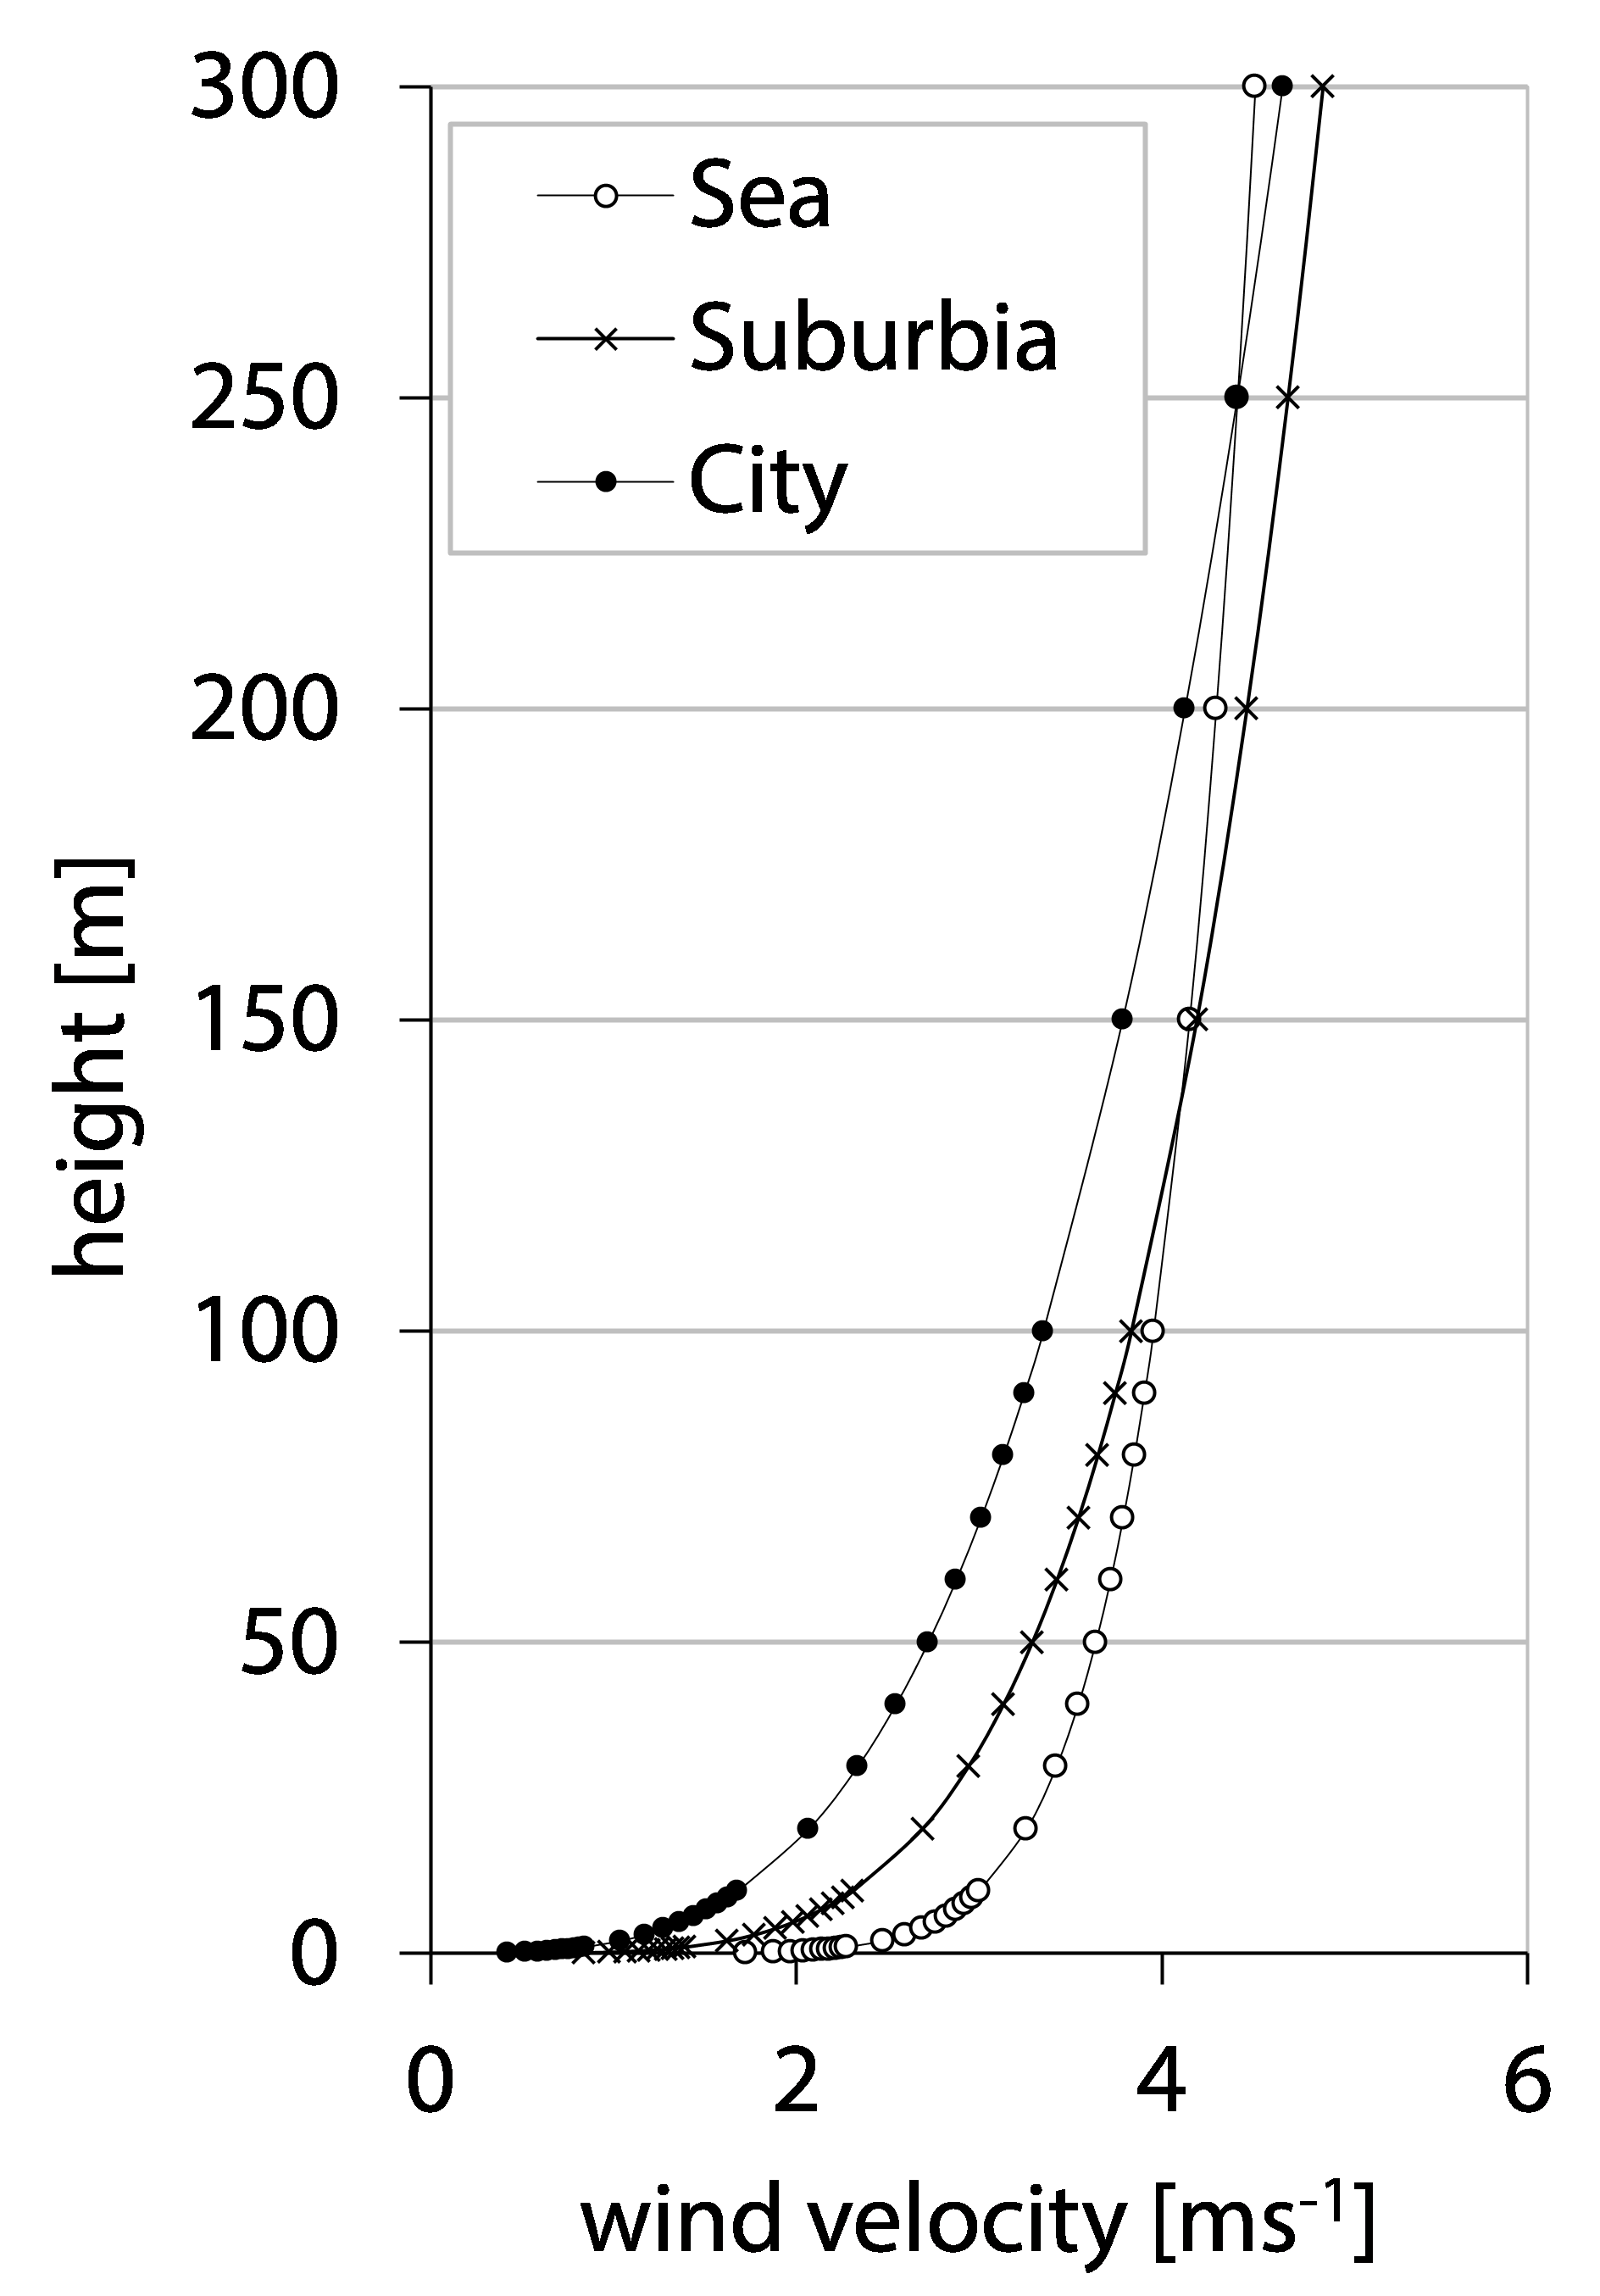
\includegraphics[height=0.4\textwidth]{images/atmospheric_boundary_layer}}
	\captionsetup{format=plain}
	\caption[Atmospheric boundary layer over three types of surface roughnesses]{Atmospheric boundary layer over three types of surface roughnesses. \textbf{(a)} The \ABL\ over city, suburbia and sea. For each surface, the plots ends when $u = \SI{4}{\metre\per\second}$ is reached. \textbf{(b)} All plots shown up to a height of $\SI{300}{\metre}$ for comparison. }
	\label{fig:theory:ABL_example}
\end{figure}

The wind shear is quantified by the exponent $\alpha$ in the power law equation \ref{eq:power_law} that relates wind velocities at two different altitudes.

\begin{equation}
u(z)=u_{ref}\left( \frac{z}{z_{ref}}\right )^\alpha
\label{eq:power_law}
\end{equation}

%\begin{itemize}
%	\item $\alpha$ is the wind shear exponent 
%	\item $z$ is the height above ground
%\end{itemize}

%where $\alpha$ is the wind shear exponent and
where $z$ is the height above the reference height. The larger the exponent $\alpha$, the larger the vertical gradient in the wind speed. This equation is accurate for altitudes from \SI{100}{\metre} up tp the top of the atmospheric boundary layer. 
For altitudes closer to the ground level, the following logarithmic relation is more applicable \citep{Ghiaus2012,Hucho2011}.

\begin{equation}
u(z) = \frac{u^*}{\kappa} ln \left( \frac{z+z_0}{z_0}\right)
\end{equation}

where \gls{symb:u*} is the \glsdesc{symb:u*}, \gls{symb:kappa} is the \glsdesc{symb:kappa} and \gls{symb:z_0} is the \glsdesc{symb:z_0}. The \glsdesc{symb:z_0}s for different terrains may be found in  \fref{tab:davenport_roughness_class} in the appendix.

Measured wind data have to be converted to a specific site, as wind data is usually collected at airport sites, which correspond to a roughness range of \SIrange{0.0024}{0.03}{} \cite{Ragheb2016}. Translation the data to a specific location is not an easy task because of the irregularities of the urban texture \citep{Ratti2002}.

%\enlargethispage*{3cm}
The \gls{DIN} \citep{DIN105542005} suggests a modified profile in which the equation is tailored to certain terrains with the help of the constant $C_{terrain}$. \Fref{tab:boundary_layer_roughness_alpha} shows certain terrain types that can be used with their own specific characteristics described.
Note that the $z_0$ values by \gls{DIN} are not consistent with the ones provided in the appendix, which stresses the point that these are empirical values. 

\begin{equation}
u(z)=C_{terrain} \cdot u_{ref}\left( \frac{z}{z_{ref}}\right )^\alpha
\end{equation}



\begin{table}[hbt]
	\small
	\centering
	\captionsetup{format=plain}
	\caption[Coefficient of terrain for different surface roughnesses]{Coefficient of terrain for different surface roughnesses. Both values are needed to transfer data in a homogeneous site \citep{DIN105542005}.}
	\label{tab:boundary_layer_roughness_alpha}
	\begin{tabular}{llSSS}
		\toprule
		Category&  	Description									& {$C_{terrain}$}   & {$\alpha$} 		& {$z_0$} \\
		\midrule
		I 	&	Sea, flat landscape             			& 1.18 				& 0.12     			& 0.01  \\ 
		II 	&	Agricultural landscape         				& 1.0  				& 0.16     			& 0.05  \\ 
		III &	Suburbia, forest              				& 0.77 				& 0.22     			& 0.3   \\ 
		IV 	&	Cities 										& 0.56 				& 0.30    			& 1.0   \\
		\bottomrule
	\end{tabular}
\end{table}


\glsresetall
\include{3_chapter}
\glsresetall
\include{4_chapter}
\glsresetall
% !TeX encoding = UTF-8
% !TeX program = lualatex
% !TeX spellcheck = en_US
% !TeX root = thesis.tex

\chapter{Validation studies}
\label{chap:validation_&_verification_study}
\index{validation}
\enlargethispage*{3cm}


\blindtext[1]

\blindtext[1]

%, which is the process of determining that the implementation of a model represents the developer's concept of the model and solution.
Thus, we use validation methods which assess to which quantifiable extent a model is able to represent reality \citep{AIAA1998}. 
%Due to time limitations and preexisting best practice guidelines for environmental flows \citep{Franke2004,Franke2006,Franke2007,Franke2010,Blocken,Ramponi2012} this chapter will focus on validation of the results, such as comparing the results with experimental data in order to quantify accuracy and errors. 
In the validation study, the following elements will be examined \citep{Slater2008,Franke2007}:

\begin{itemize}
%	\item Comparison against experimental datak
	\item Implementation of the model
	\item Consistency
	\item Mesh refinement  
	\item Iterative convergence
	\item Spatial convergence	
	\item Sensitivity of boundary conditions	
\end{itemize}




\enlargethispage*{3cm}
\begin{figure}[!h]
	\centering
	\subfloat[][Residuals very coarse]%
	{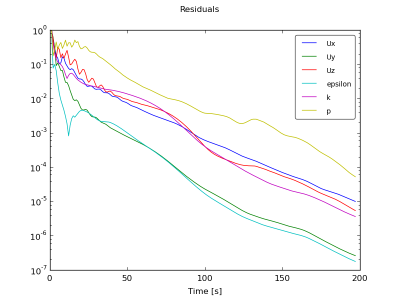
\includegraphics[width=0.48\textwidth, trim= 14mm 2mm 12mm 17mm, clip]{images/plots/validation/iterative_convergence/linear_very_coarse}}\hfil
	\subfloat[][Residuals coarse]%
	{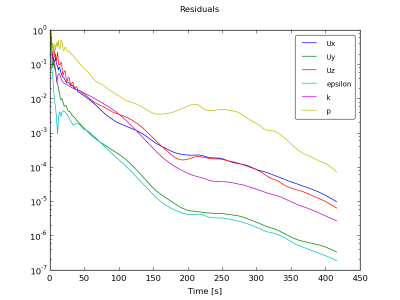
\includegraphics[width=0.48\textwidth, trim= 14mm 2mm 12mm 17mm, clip]{images/plots/validation/iterative_convergence/linear_coarse}}\hfil
	\subfloat[][Residuals normal]%
	{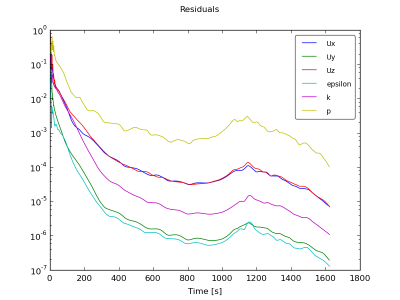
\includegraphics[width=0.48\textwidth, trim= 14mm 2mm 12mm 17mm, clip]{images/plots/validation/iterative_convergence/linear_ref}}\hfil
	\subfloat[][Residuals fine]%
	{\begin{annotatedFigure}
			{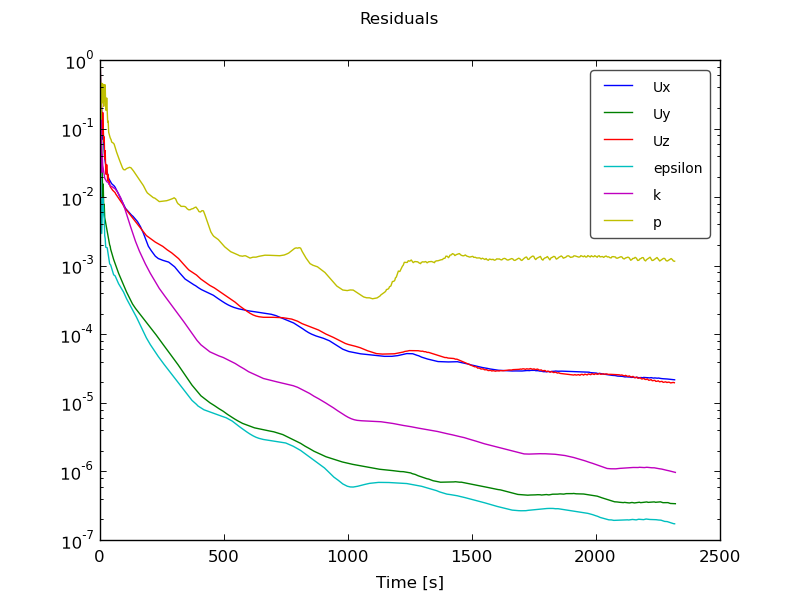
\includegraphics[width=0.48\textwidth, trim= 14mm 2mm 12mm 17mm, clip]{images/plots/validation/iterative_convergence/linear_fine}}
			\annotatedFigureBoxBlack{0.47,0.57}{0.89,0.65}{A}{0.47,0.57}%bl
	\end{annotatedFigure}}\hfil
	\centering
	\subfloat[][Volumetric flow rates obtained by the meshes above. The flow rate in the experiment was measured as \SI{0.045}{\cubic\metre\per\second}.]%
	{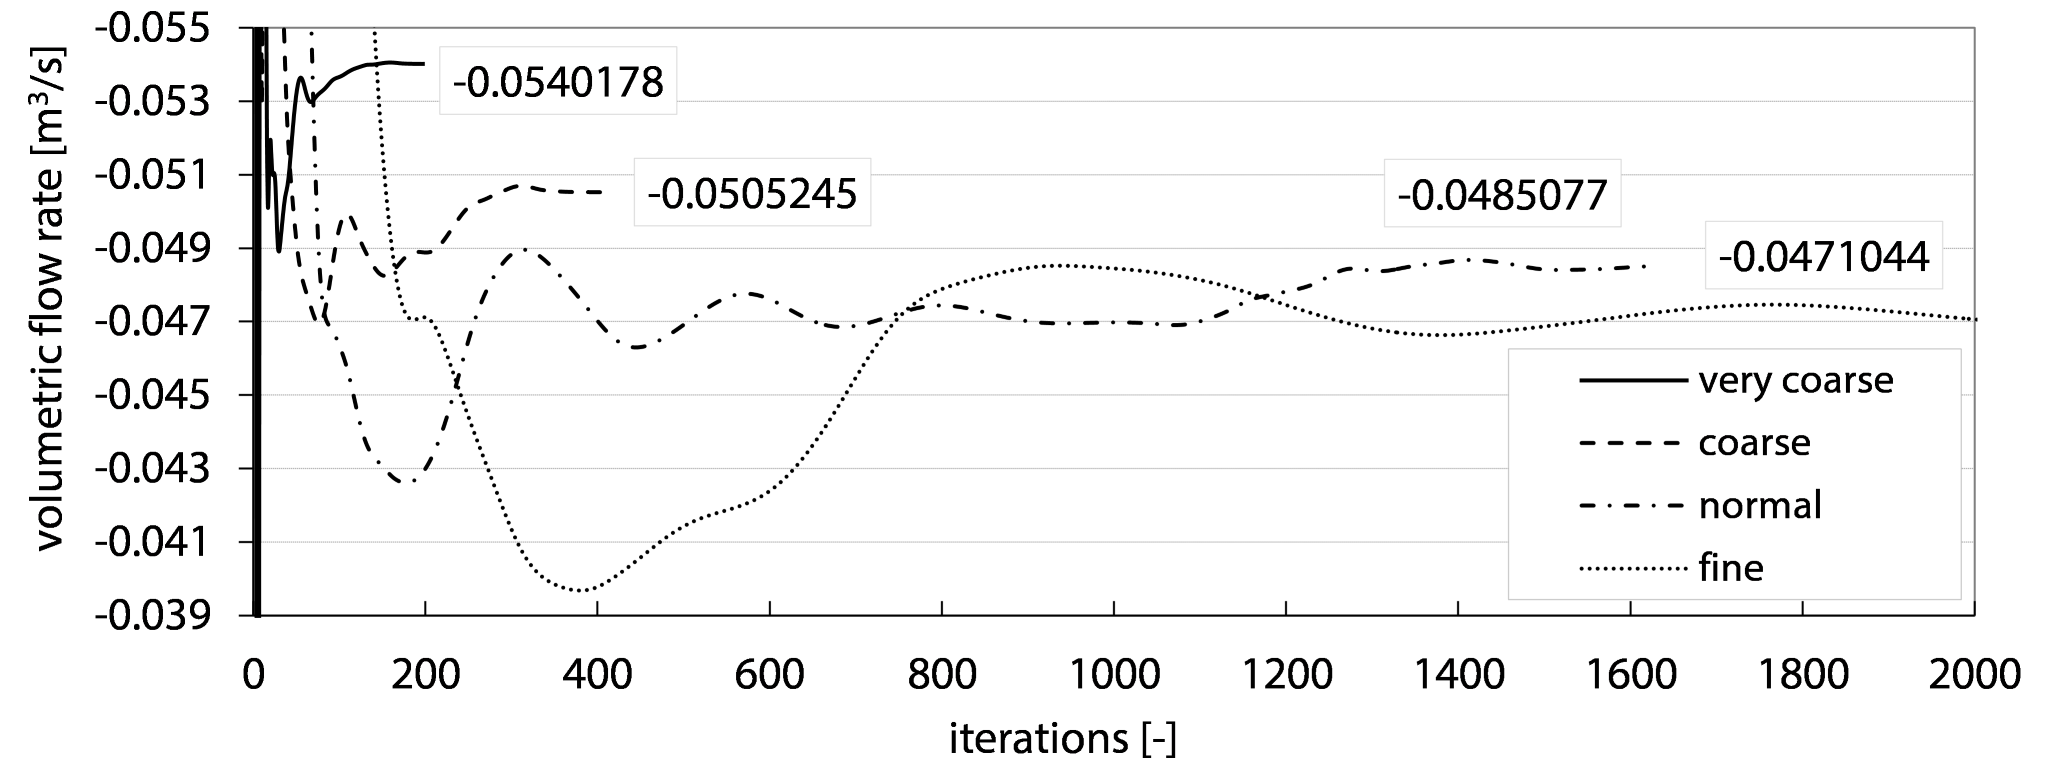
\includegraphics[width=1\linewidth, trim= 14mm 11mm 12mm 7mm, clip]{images/plots/validation/volumetric_flow_rates_grid_study}}
	\captionsetup{format=plain}%,labelsep=newline}
	\caption[Residual plots and volumetric flow rates of the mesh refinement study]{Residual plots and volumetric flow rates of the mesh refinement study. \textbf{(a-c)} The finer the mesh, the more iterations are needed to until the convergence criteria is reached. \textbf{(d)} The residuals of the \textit{fine} mesh did not reach the convergence criteria and showed oscillatory convergence for the pressure variable, see \textbf{(A)}. \textbf{(e)} Volumetric flow rates obtained by the aforementioned meshes. The convergence criteria in \fref{tab:convergence_crit_validation_study} are stringent enough to obtain stable solutions with regard to volumetric flow rates.}
	\label{fig:validation:residual_plots+volumetric_flow rates}
\end{figure}




Finally, the \textit{potentialFoam} solver should be implemented in the work-flow, which could not be done in this thesis in the interest of time.
The \textit{potentialFoam} solver provides initial fields by only solving the pressure equation of the \gls{NSE}.
Thus, it can be used as an efficient solver, initializing the velocity field for more complex solvers like \textit{simpleFoam}. 
As a result, instead of starting from a resting flow with \textit{simpleFoam}, the \textit{potentialFoam} solution may be used as an initial guess and to help to achieve convergence faster.



\FloatBarrier

%Grid study showing the discrepancies between various grids \cite{Ramponi2012}
%\clearpage
\subsubsection{Spatial convergence}
\label{sec:validation:spatial_convergence}
\index{validation!spatial convergence}

In this section, the 4 stages of mesh refinement discussed in \fref{sec:validation:mesh_fineness} are used to determine whether spatial convergence is obtained.
In doing so, one is able to determine up to which extent the mesh should be refined to ensure that  the result for a derived variable (such as the flow rate) will not change significantly with further iterations.

Along with this, another method that falls under the spatial convergence assessment method is called \gls{RE} \citep{Slater2008}. 
It predicts the variable of interest for a theoretically perfect grid with zero grid spacing\textemdash essentially a continuum\textemdash by using lower-order discrete values of that same variable.

Moreover, one is able to estimate the numerical discretization error caused by various mesh sizes. 
This allows to estimate the error due to discretization altogether. 
\Fref{tab:grid_convergence_study} shows the parameters of the 4 mesh sizes studied. 


\definecolor{light-grey}{cmyk}{0,0,0,0.10}

\begin{table}[!b]
	\footnotesize
	\centering
	\captionsetup{format=plain}
	\caption[Parameters of grid convergence study]{Parameters of grid convergence study. The study was conducted for 4 different mesh sizes: \textit{very coarse}, \textit{coarse}, \textit{normal} and \textit{fine}.  $r$ is the grid refinement ratio and $h$ is the normalized  grid spacing. Moreover, the Richardson Extrapolation (RE) predicts the flow rate for an ideal mesh (continuum), estimating the magnitude of the numerical error. $\dot{v}$ shows the flow rate through the windward opening obtained.  exp. $=$ experiment by  \citep{Jiang2003}. cont. $=$ continuum. The \textit{normal} mesh shows reasonable accuracy and is therefore chosen for further studies.}
	\label{tab:grid_convergence_study}
	\begin{tabular}{SrlrSSSSSS}
		\toprule
		{\#} & type & case                            & {cell \#} 	    & {$h$} & {$r$}  &  {$\dot{v}$ [\si{\cubic\metre\per\second}]}  & {error (exp.)} &  {error (cont.)}  &\\ \midrule
		1   &  sim.  & very coarse                 & \num{124456}     	& 8   	& 1.3 	& 0.054	& \SI{17}{\percent}  & \SI{15}{\percent} &\\%0.054017
		2   &  sim.  & coarse                        & \num{263919}     	& 4   	& 1.6 	& 0.051	& \SI{11}{\percent}  & \SI{10}{\percent}&\\%0.050524
		\rowcolor{light-grey}  3   & sim.    & normal                        & \num{1165733}   	& 2   	& 1.6 	& 0.049	&\SI{7}{\percent}   & \SI{6}{\percent}&\\%0.048507
		4   & sim.   & fine                             & \num{4940280}  	& 1   	& {-} 		& 0.047	& \SI{4}{\percent}  & \SI{3}{\percent} &\\%0.047104
		{-}  &  calc.  & RE                              & {-}       		& 0   	& {-} 		& 0.046	&  &\\%0.045752
		{-}  &  meas.  & experiment  & {-}       		& {-} 		& {-}  	& 0.045 &  &\\ \bottomrule
	\end{tabular}
\end{table}



The effective grid refinement ratio $r$ for unstructured grids is defined as:

\begin{equation}
r = \left( \frac{N_{i}}{N_{i+1}}\right)^\frac{1}{D} 
\end{equation}




\glsresetall
% !TeX encoding = UTF-8
% !TeX program = lualatex
% !TeX spellcheck = en_US
% !TeX root = thesis.tex

\chapter{Case study - BRAC University}
\label{chap:case_study_BRAC_U}
\index{BRAC}


\blindtext[2]



\begin{figure}[hbt]
	\centering
	\includegraphics[width=0.9\linewidth]{images/BRAC_Model}
	\caption[BRAC University]{BRAC University \cite{WOHA}.}
	\label{fig:bracmodel}
\end{figure}





\clearpage

\thispagestyle{empty}
\vspace*{\fill}
\begin{center}
\sffamily This page is intentionally left blank
\end{center}
\vspace*{\fill}


\clearpage

%\newpage
\paragraph{Reference layout}

To start with, the results of the reference layout V1-4w will be discussed with regard to conventional visualization techniques.
%In this section, the simulation results for BRAC University regarding \ACR s and CO$_2$ concentration as well as age of air are going to be shown and discussed.
All following horizontal cross-sections are taken at (\SI{1.35}{\metre}) above the floor and clipped to the size depicted in the figures. It should  also be noted that the \ACR\ illustrations are not true to scale and solely serve the purpose of depicting the geometric features. For true scale geometries please refer to \fref{sec:appendix:BRAC_geometry}.

\Fref{fig:V1-4w_flow_field} illustrates the horizontal cross-section\footnote{Note that horizontal cross-sections of $|u|$ are instantaneous snapshots of the flow field. A visual examination against iteration-averaged values did not show different flow characteristics.} of V1-4w colored by $|u|$. This visualization is a conventional method of illustrating a flow field.
The flow is characterized by the following characteristics:

\begin{enumerate}[label=(\Alph*)]
	
	\item Flow separation with a reattachment point of approximately \SI{30}{m} into the building block.
	
	\item  Constriction of the flow in staircase area; following the continuity constraint,  the velocities increased by a factor of $\sim$\num{2}.
	
	\item Local velocity differences that create vortices in the windward \CR.
	
	\item  Indefinite flow structure in leeward \CR s where the ventilation pattern changes from a \CR\ of type (C) to (D).
	
\end{enumerate}





\begin{figure}[!hb]
	\centering
	\subfloat[][conventional flow field]{
	\begin{annotatedFigure}{
			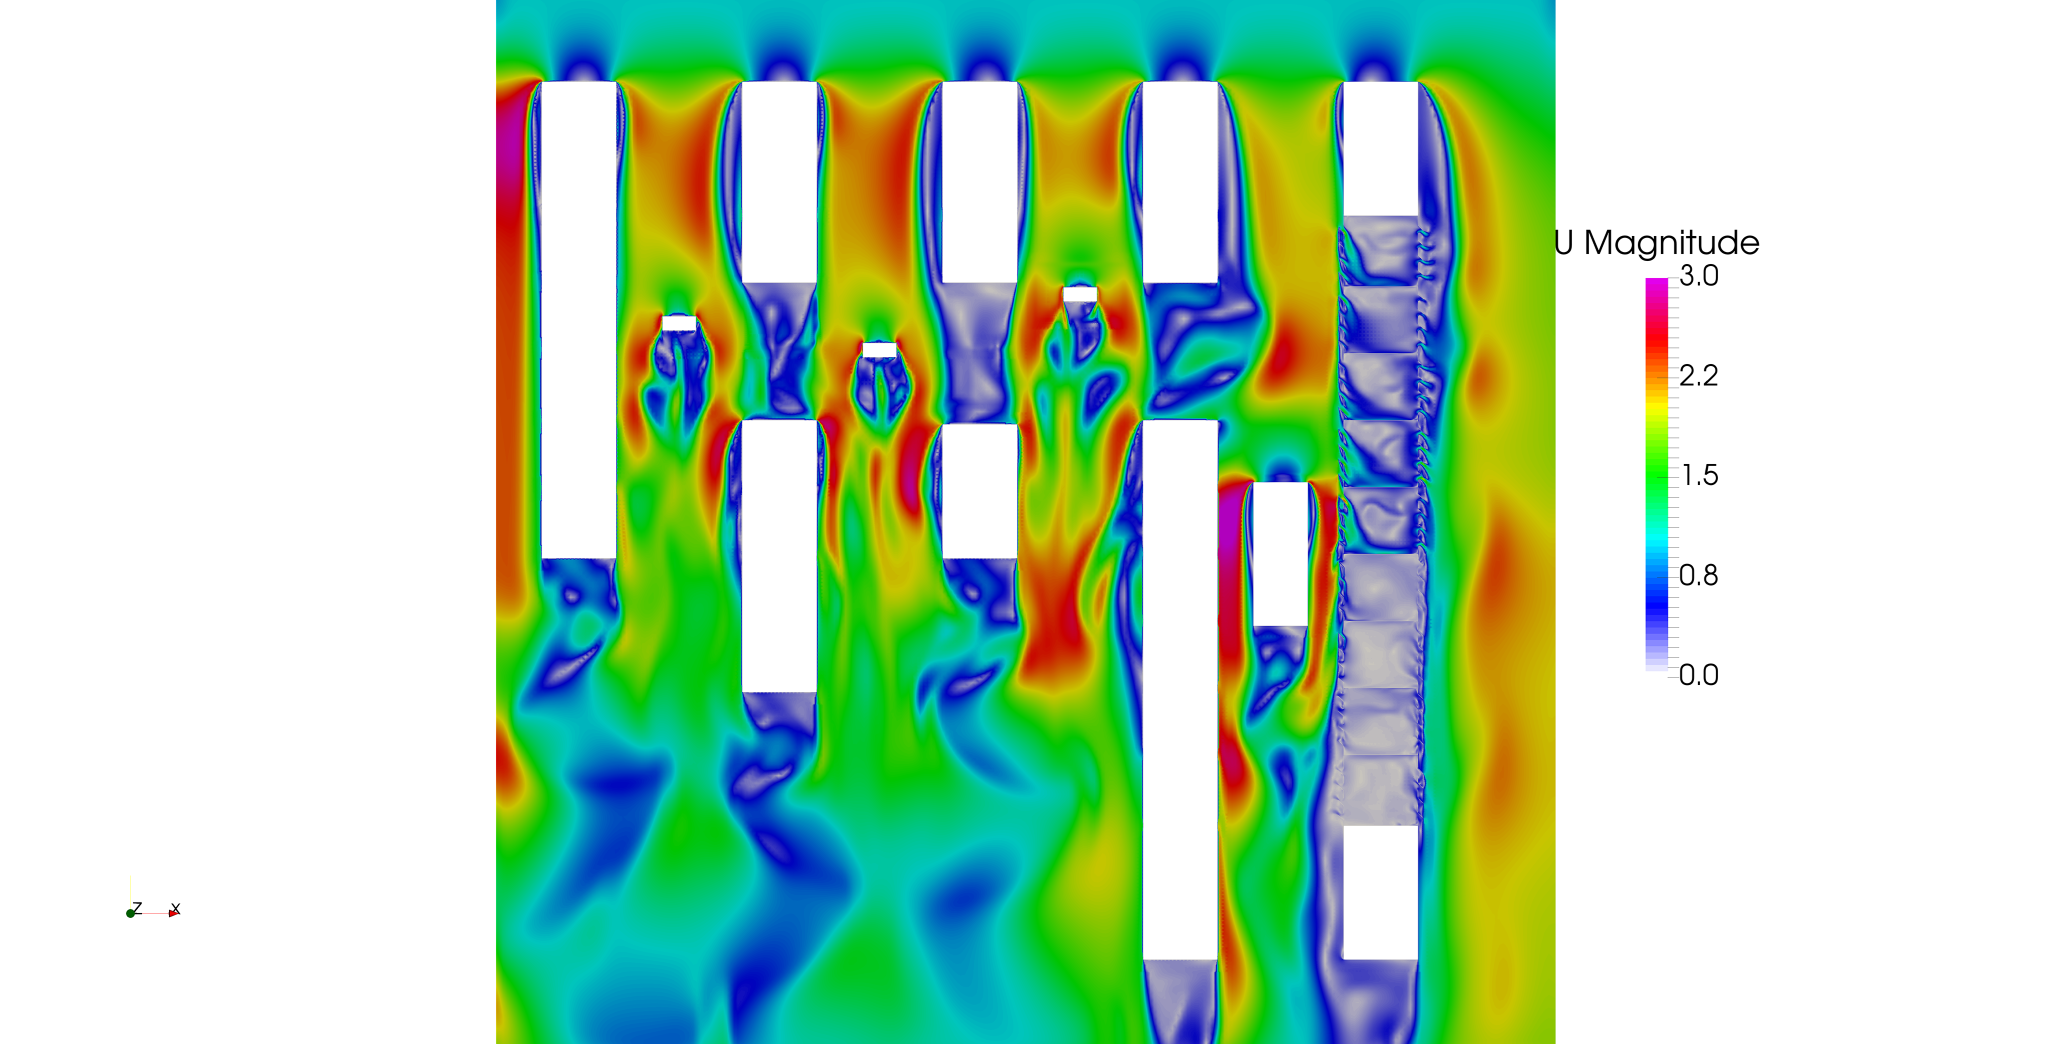
\includegraphics[width=0.35\linewidth, trim= 86cm 10cm 35cm 2.5cm, clip]{images/topview/V1-4w/topview_magU}}
		\annotatedFigureBox{0.2,0.85}{0.90,0.95}{A}{0.2,0.85} 	
		\annotatedFigureBox{0.02,0.27}{0.38,0.51}{B}{0.02,0.25} 
		\annotatedFigureBox{0.33,0.55}{0.63,0.65}{C}{0.33,0.55} 	
		\annotatedFigureBox{0.25,0.09}{0.63,0.25}{D}{0.25,0.09} 		
		%(links , unten)	(rechts, oben)
	\end{annotatedFigure} \hspace*{0.2cm}
	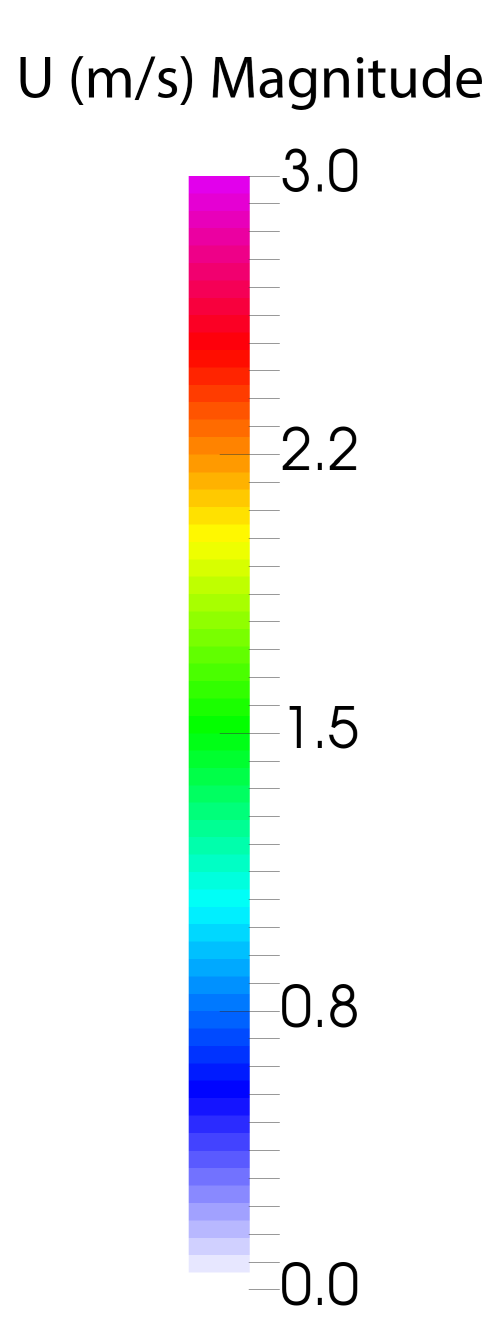
\includegraphics[width=0.25\linewidth, trim= -5cm -14cm 0cm 0cm, clip]{images/topview/scale_magU}}
	%	\hspace*{3cm}\llap{\raisebox{1cm}{%minus raisebox schibet nach unten
	%			%	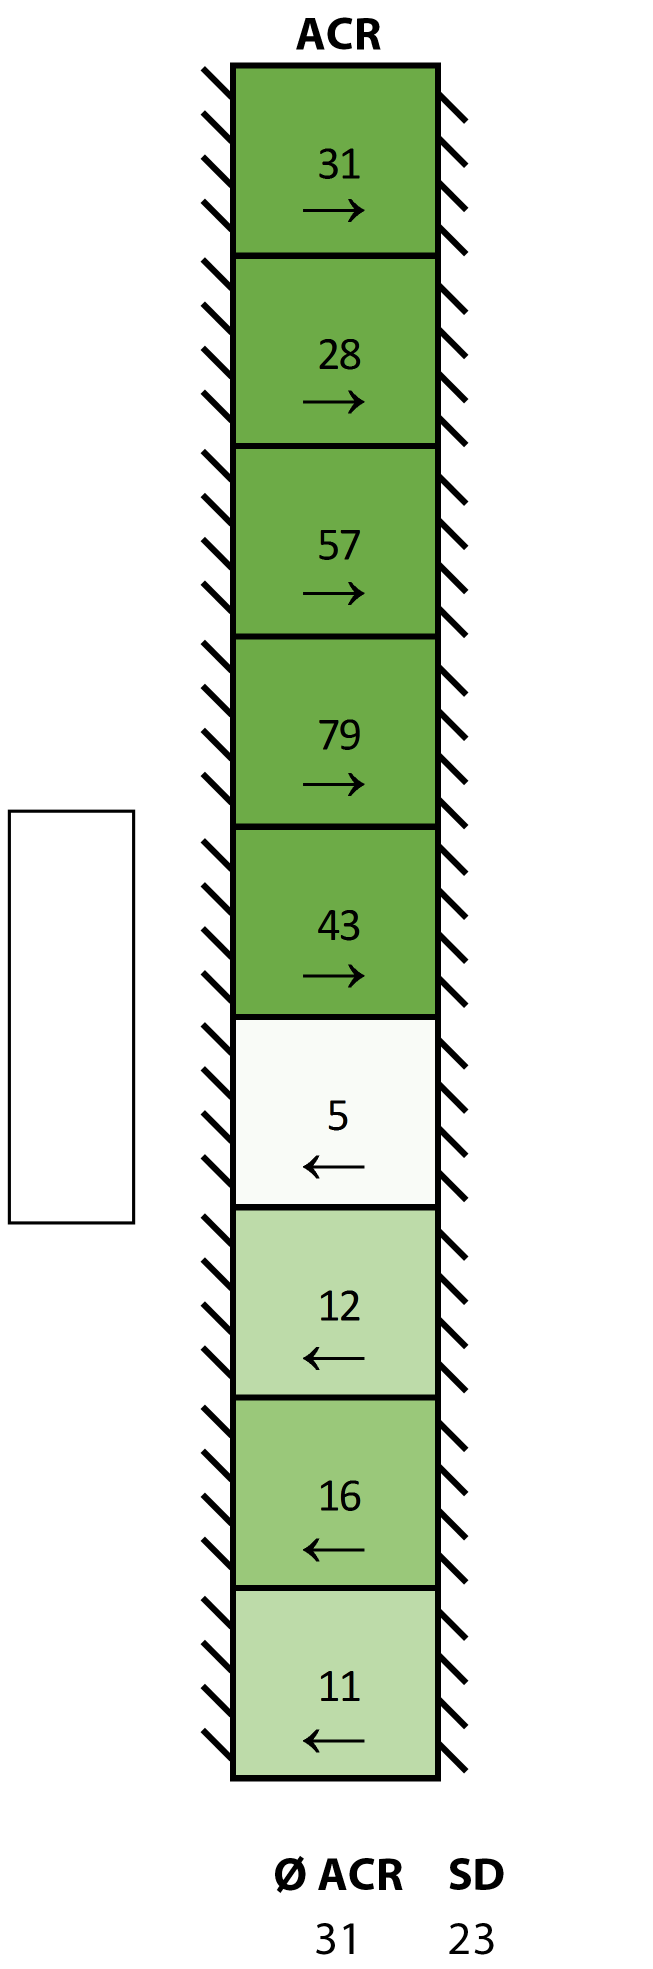
\includegraphics[width=0.14\linewidth, trim= 1.4cm 1cm 1.4cm 0.45cm, clip]{images/ACR/ACR_V1-4w}	
	%	}}
	\begin{tikzpicture}[remember picture, overlay]
	\node[yshift=8cm] {\includegraphics[scale=0.3, trim= 0cm 0cm 0cm -2cm, clip]{images/arrow_N}};
	\end{tikzpicture}
	\subfloat[][ACRs]{	
	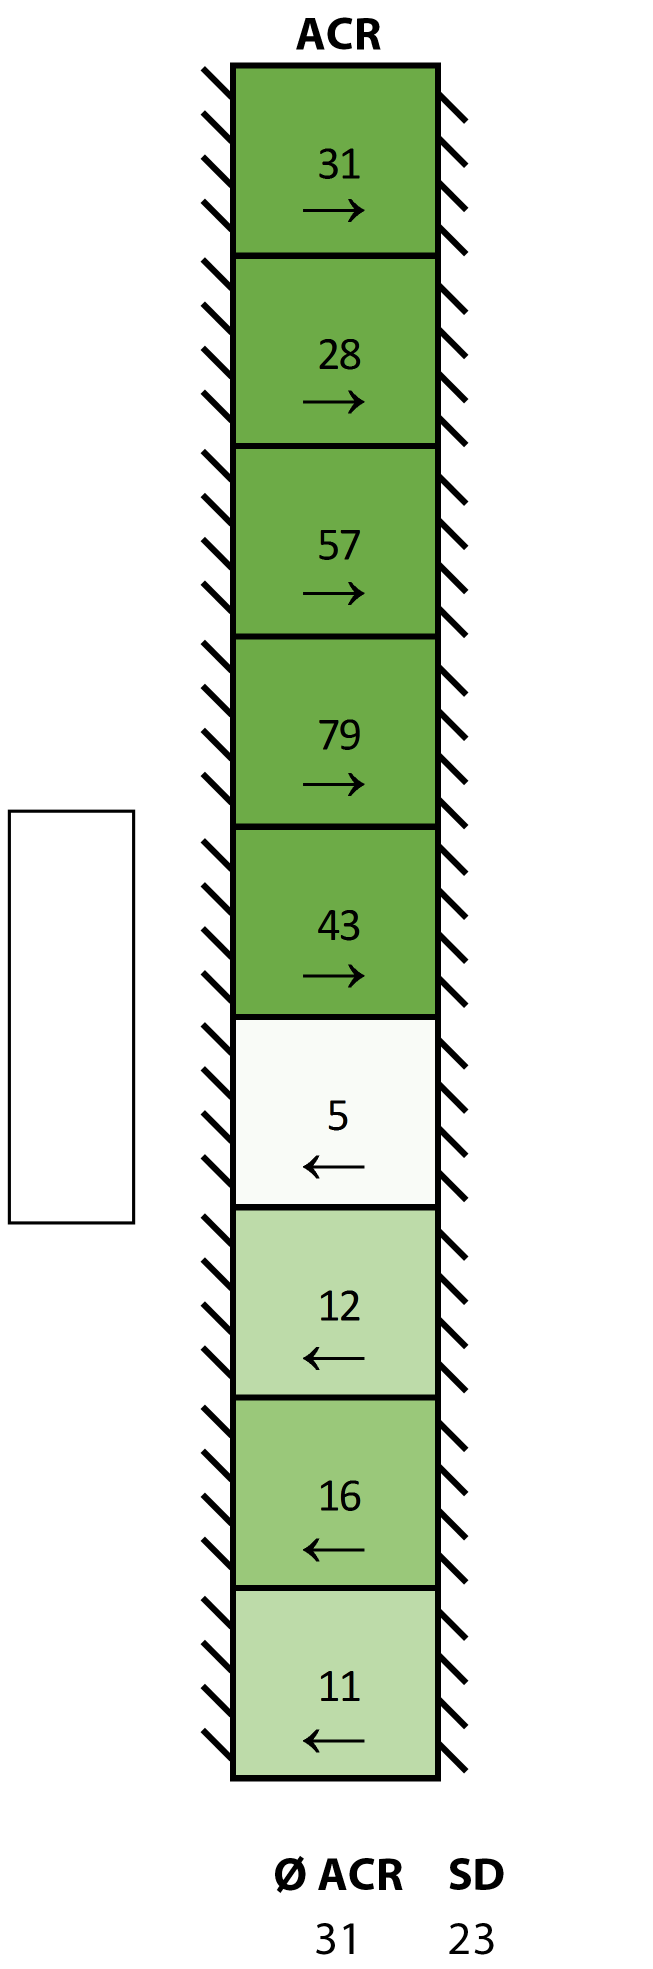
\includegraphics[width=0.14\textheight, trim= 0.00cm -2.7cm 5cm 0.45cm, clip]{images/ACR/ACR_V1-4w}}	
	\captionsetup{format=plain}
	\caption[Flow characteristics of V1-4w]{Horizontal cross-section of V1-4w depicting  $|u|$ and the flow characteristics. (\textbf{A}) Flow separation occurs in the area of the windward building block with a reattachment point of about \SI{30}{m}. (\textbf{B}) Constriction of the flow in the area of the staircase; following the continuity constraint,  the velocities increase by a factor of $\sim$\num{2}. (\textbf{C}) Local velocity differences create vortices in the windward \CR. (\textbf{D}) Indefinite flow structure in leeward \CR; the ventilation direction changed from \CR\ type (C) to type (D).}
	\label{fig:V1-4w_flow_field}	
\end{figure}
\enlargethispage*{1.0cm}



\index{BRAC!air change rates}

\blindtext[1]

\blindtext[1]


\cleartoleftpage

\subsubsection{Impact of the number of windows}
\index{BRAC!effects!number of windows}
\enlargethispage*{4cm}

\blindtext[1]


\paragraph{Air change rates}

\blindtext[1]


\paragraph{CO$_2$ concentration}

\blindtext[1]


\paragraph{Age of air}

\blindtext[1]




\begin{figure}[!htbp]
	%	\centering \hspace*{-2cm} 
	\begin{tikzpicture}[remember picture, overlay]
	\node[yshift=8cm] {\includegraphics[scale=0.3, trim= 0cm 0cm 0cm -2cm, clip]{images/arrow_N}};
	\end{tikzpicture}
	\subfloat[][V1-4w]%
	{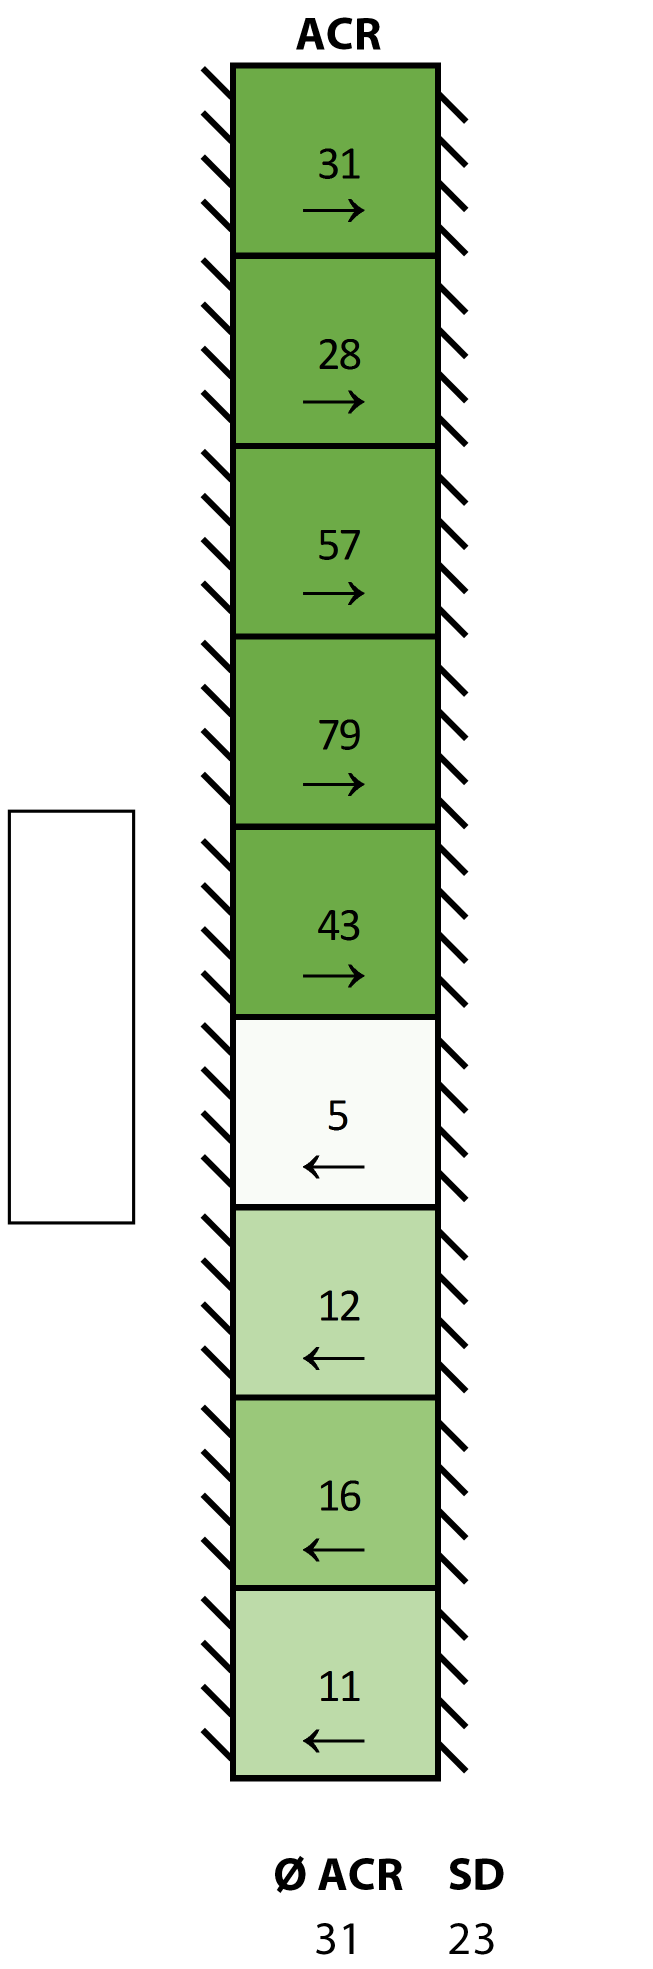
\includegraphics[width=0.135\textheight, trim= 0.00cm 0.1cm 5cm 0.45cm, clip]{images/ACR/ACR_V1-4w}\hspace*{0.5cm}
		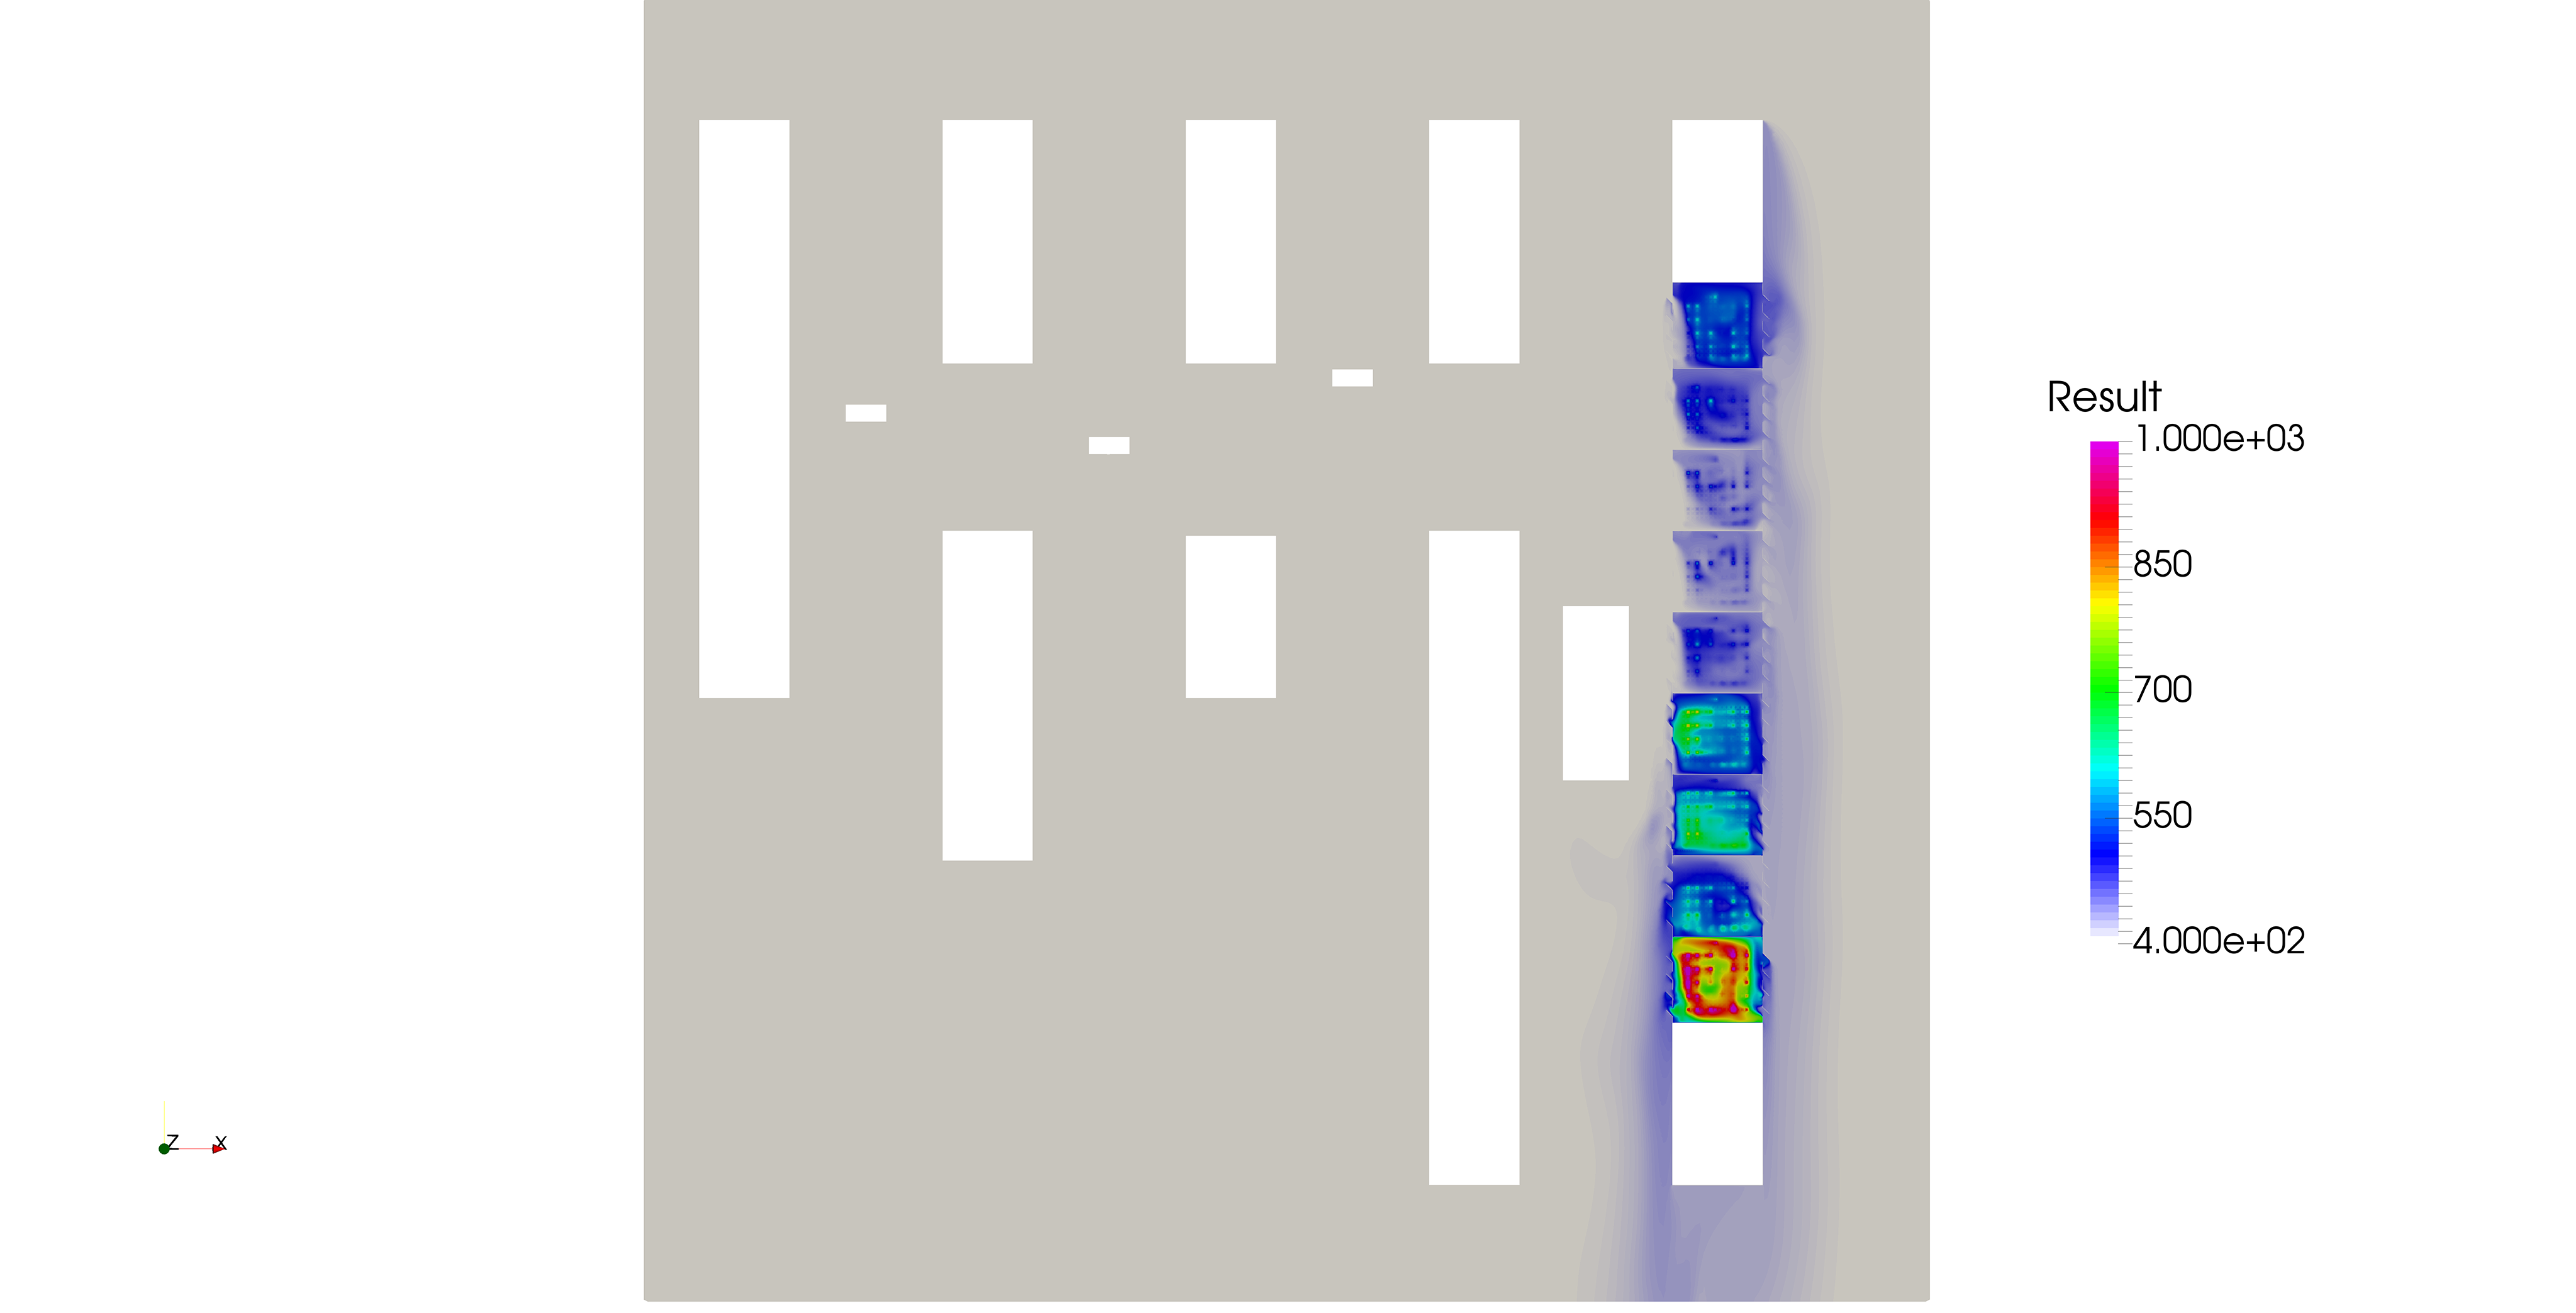
\includegraphics[width=0.162\textheight, trim= 86.5cm 11.5cm 41cm 15cm, clip]{images/CO2/V1-4w/topview_CO2}}
	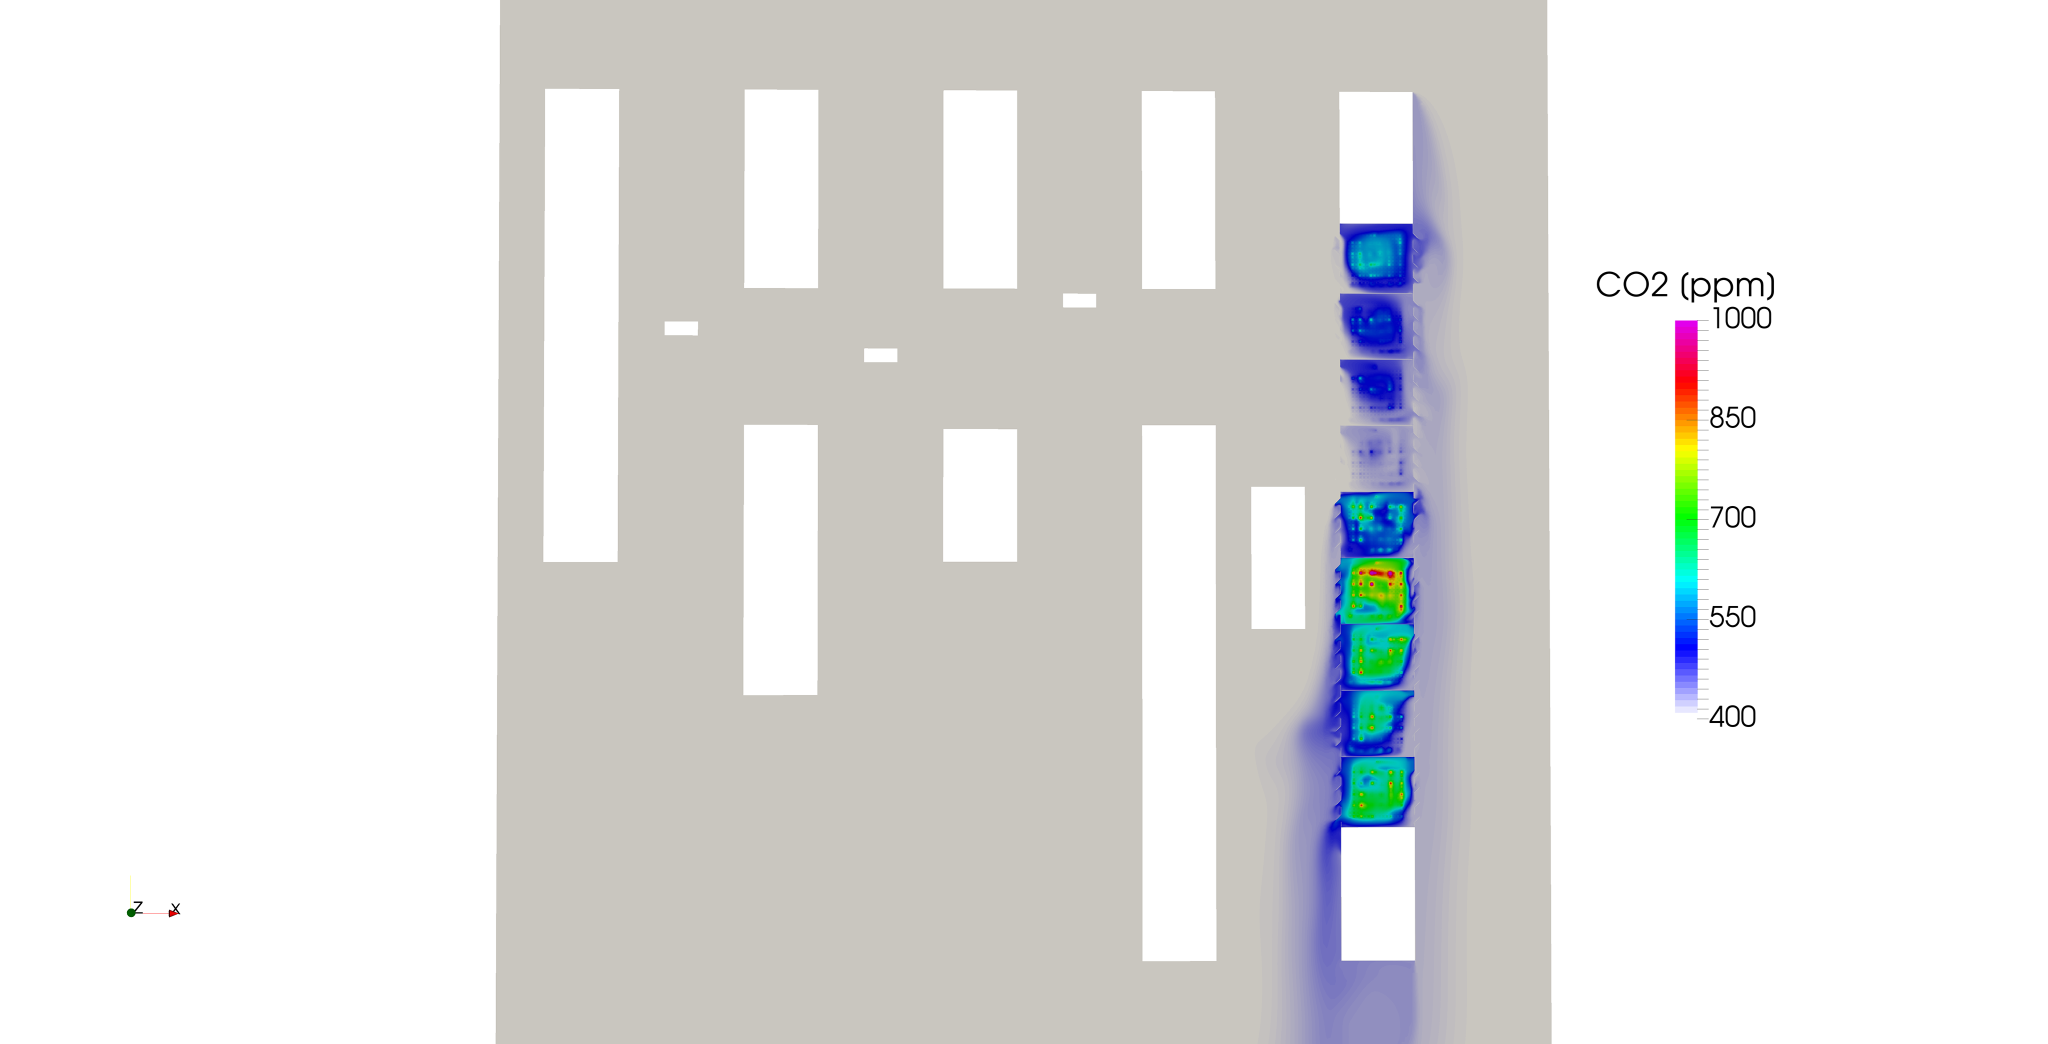
\includegraphics[width=0.09\textheight, trim= 112cm 5.85cm 19cm 10cm, clip]{images/CO2/V0/topview_CO2}\hspace*{0.5cm}
	\includegraphics[width=0.062\textheight, trim=65cm -8cm 68cm 0cm, clip ]{images/AoA/BRAC/V1-4w/topview_AoA4}
	\includegraphics[width=0.062\textheight, trim=90cm 7cm 45cm 0cm, clip ]{images/AoA/BRAC/V1-4w/topview_AoA4}  \\
	\begin{tikzpicture}[remember picture, overlay]
	\node[yshift=8cm,xshift=-3.2cm] {\includegraphics[scale=0.3, trim= 0cm 0cm 0cm -2cm, clip]{images/arrow_N}};
	\end{tikzpicture}
		\subfloat[][\mbox{V1-1w}]		
	{\hspace*{-3.2cm}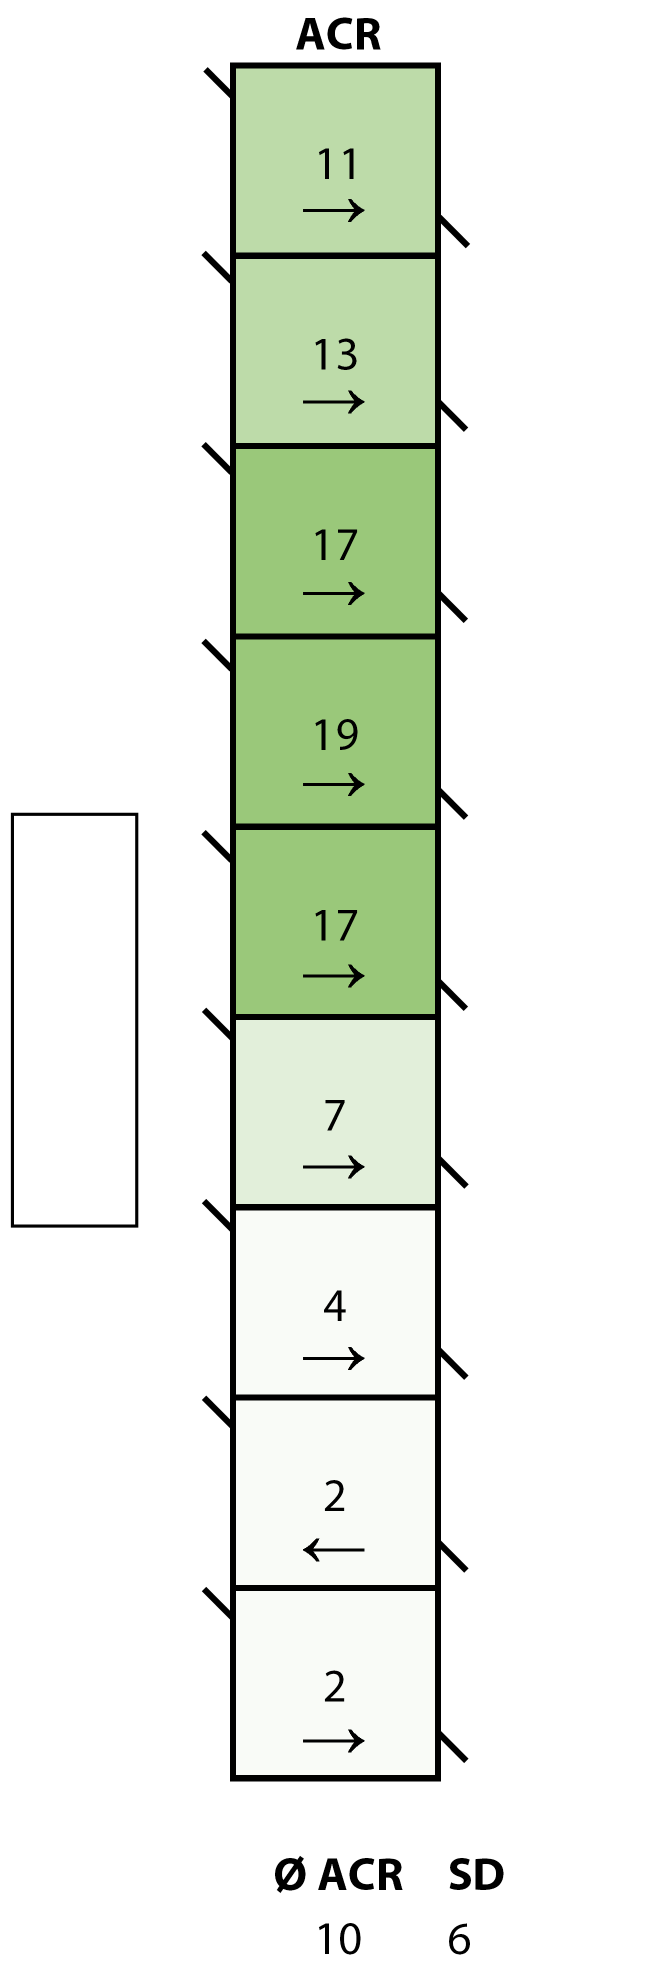
\includegraphics[width=0.135\textheight, trim= 0.00cm 0.1cm 5cm 0.45cm, clip]{images/ACR/ACR_V1-1w}}\hspace*{0.1cm}
	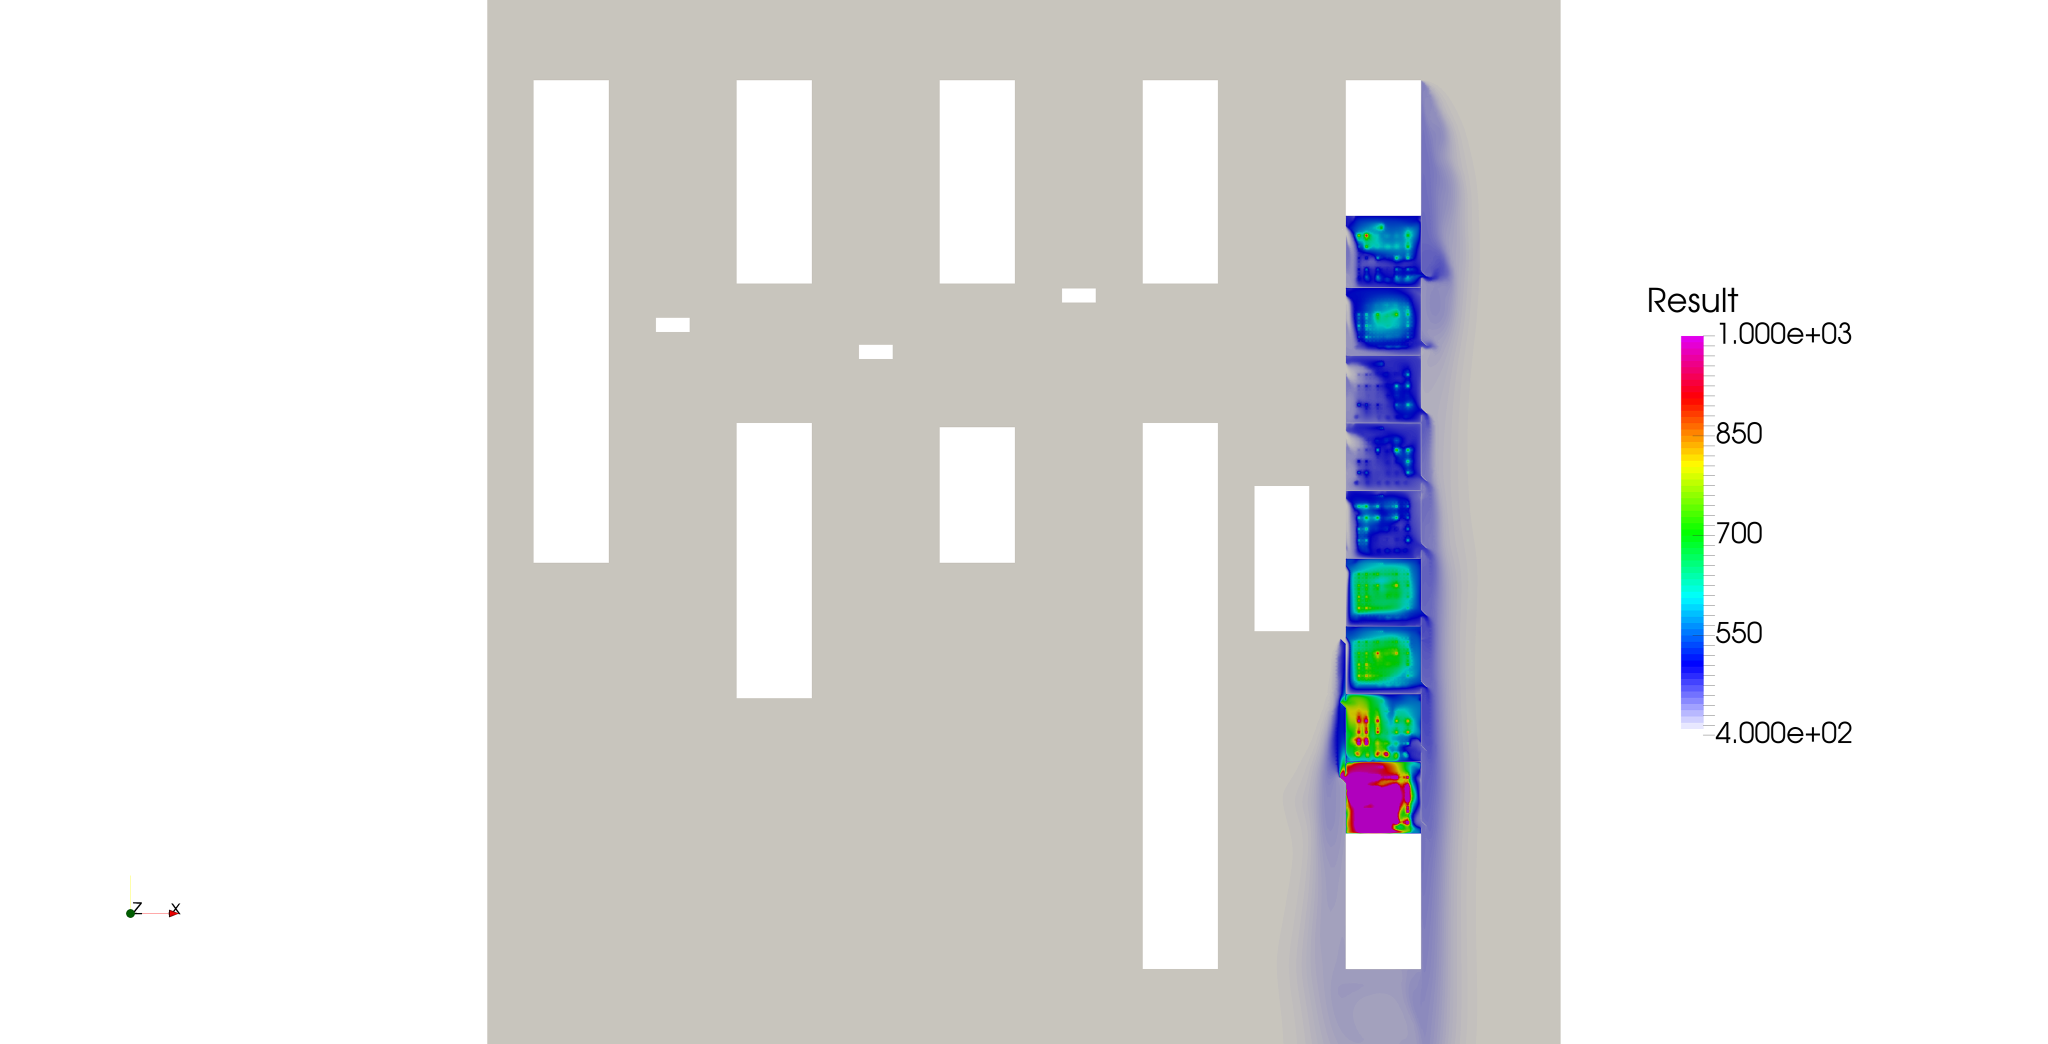
\includegraphics[width=0.160\textheight, trim= 86.5cm 11.5cm 41cm 15cm, clip]{images/CO2/V1-1w/topview_CO2}
	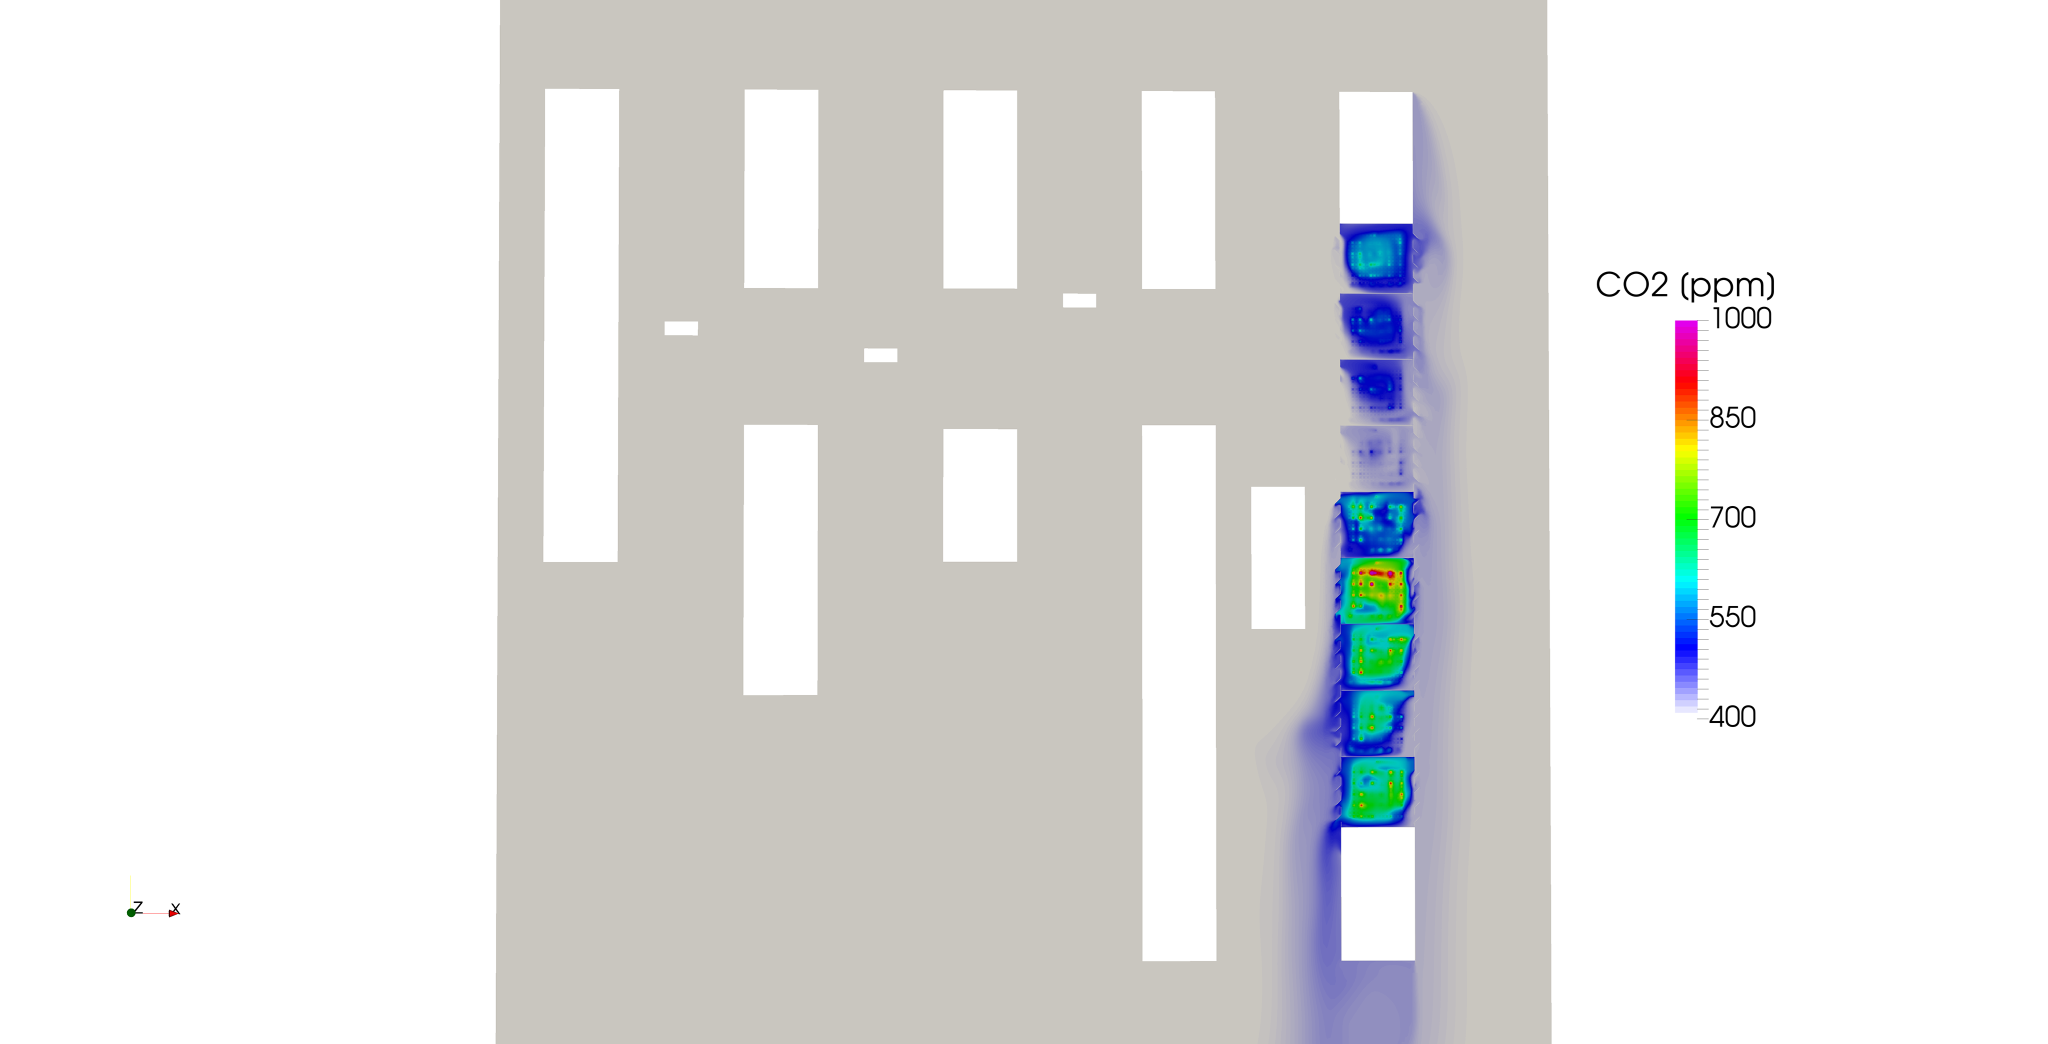
\includegraphics[width=0.09\textheight, trim= 112cm 5.85cm 19cm 10cm, clip]{images/CO2/V0/topview_CO2}
	\captionsetup{format=plain}
	\caption[Comparison of the  natural ventilation potential of V1-4w against V1-1w]{Comparison of the  natural ventilation potential of V1-4w against V1-1w. This allows us to draw conclusions how much influence the number of openings has on the natural ventilation potential.}
	\label{fig:ACR_V14w_V12w_V11w}
\end{figure}




\glsresetall
\include{7_chapter}

\small
{\pagestyle{thesisLISTS}
\listoffigures
\listoftables
%\listoflistings
\clearpage}


\clearpage
{\pagestyle{thesisINTRO}
\small
\bibliography{literature/literature}
\addcontentsline{toc}{chapter}{Bibliography}
\clearpage}

%Appendix
\normalsize
{\pagestyle{thesisAPPENDIX}
\phantomsection
\appendix
% !TeX encoding = UTF-8
% !TeX program = lualatex
% !TeX spellcheck = en_US
% !TeX root = thesis.tex

\chapter{Geometric models}
\label{chap:geometric_models}

The following pages contain the various geometry models used for both the validation study as well as BRAC University. The description of the validation study is to be found in \fref{chap:validation_&_verification_study}, the study for BRAC University in \fref{chap:case_study_BRAC_U}.




\clearpage




\begin{figure}[!h]
	\section{Validation study}
	\centering
	\includegraphics[height=1.5\linewidth, trim = 0cm 5cm 10cm 2cm ,clip]{images/geometry/validation/Validation_scaled_down_4P}
	\captionsetup{format=plain}	
	\caption[Geometry used for the validation study; top-view and front-view]{Geometry used for the validation study. Top-view and front-view of validation domain. The dimensions are given in \si{\metre}.}
	\label{fig:validationscaleddown4p}
\end{figure}



\begin{figure}[!h]
	\centering
	\subfloat[][]{
		\includegraphics[width=1\linewidth, trim = 4cm 10cm 2.5cm 11cm , clip, angle= -0.5]{images/geometry/validation/Validation_scaled_down_domain}}\\
	\subfloat[][]{
		\includegraphics[width=.6\linewidth, trim = 5cm 8.5cm 4cm 12cm , clip]{images/geometry/validation/Validation_scaled_down_building}}
	\captionsetup{format=plain}	
	\caption[Geometry used for the validation study; perspective views]{Perspective views of validation geometry  \citep{Jiang2003}. \textbf{(a)} Perspective view of the simulation domain and the vertical samples used; \textbf{(b)} The dimensions of the building within the domain are given in \si{\metre}.}
	\label{fig:validationscaleddownbuilding}
\end{figure}




\clearpage
\chapter{Validation study}
\section{Turbulence models}
\label{sec:appendix_turbulence_study}


The full samples of the validation study of different turbulence models are shown on the following pages.
For the full description of the study, the reader is referred to \fref{sec:validation_turbulence_modelling}. The general boundary conditions of the model can be found in \fref{tab:boundary_conditions_validation_study}.





%\cleardoublepage
\cleartoleftpage
\enlargethispage{3cm}
\includepdf[pages=4,clip,trim=0cm 1cm 21cm -1cm,,noautoscale,fitpaper=false, pagecommand*={\subsection{\kEps\  model}\label{app:plots:kEps}\thispagestyle{plain}\null\vspace*{20cm}\captionof{figure}{\kEps\  turbulence model}}]{images/plots/validation/validation.pdf}
\includepdf[pages=4,clip,trim=21cm 1cm 0cm -1cm,,noautoscale,fitpaper=false, pagecommand={} ]{images/plots/validation/validation.pdf}
%\captionof{figure}{Graphical Illustration of Dataset with an Arbitrary Caption to Highlight the Problem}
\clearpage



\clearpage

\begin{figure}[htbp]
	\section{Mesh refinement}
	\index{validation!LIC}
	\center \hfill 
	
\includegraphics[height=4cm, trim= -1cm 0cm 0cm 0cm, clip]{images/validation/refinement/mod/case_ultra_coarse}
	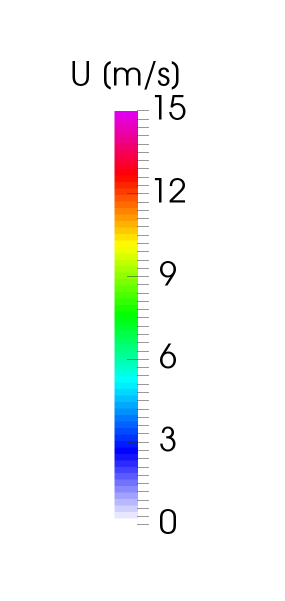
\includegraphics[width=0.15\linewidth]{images/validation/refinement/mod/scale_U}	
	\hfill 
	\noindent\parbox[b][4cm][c]{2cm}{
		\subfloat[\mbox{very coarse}]{}
	} \vspace*{0.5cm}   \\  \hfill 
	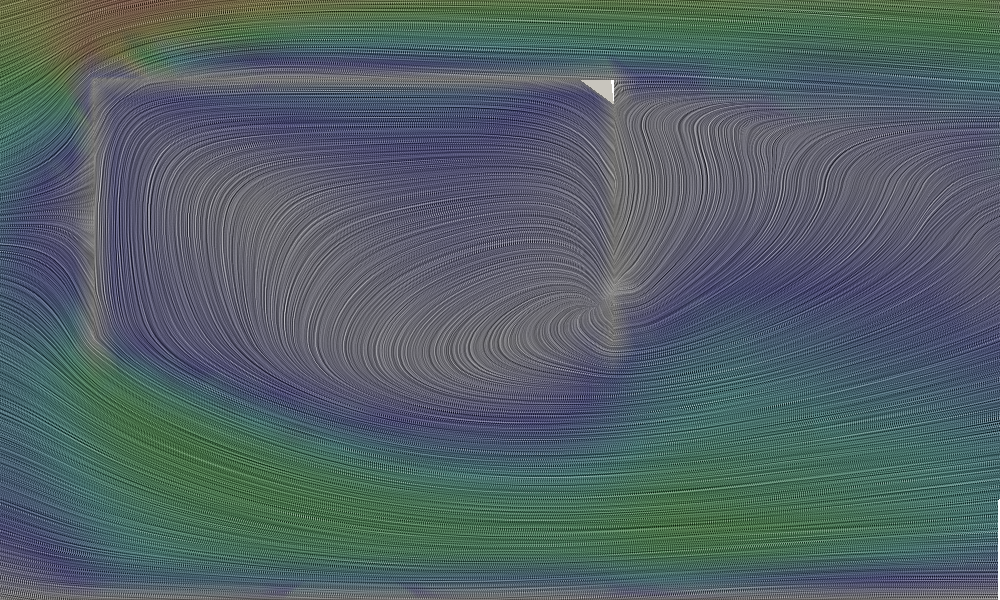
\includegraphics[height=4cm]{images/validation/refinement/mod/case_coarse}
	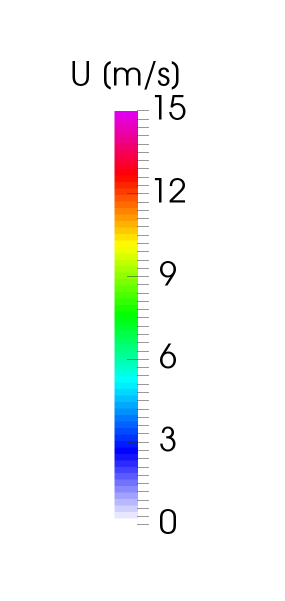
\includegraphics[width=0.15\linewidth]{images/validation/refinement/mod/scale_U}
	\hfill 
	\noindent\parbox[b][4cm][c]{2cm}{
		\subfloat[coarse]{}
	}\vspace*{0.5cm}   \\ \hfill 
	\begin{annotatedFigure}
		{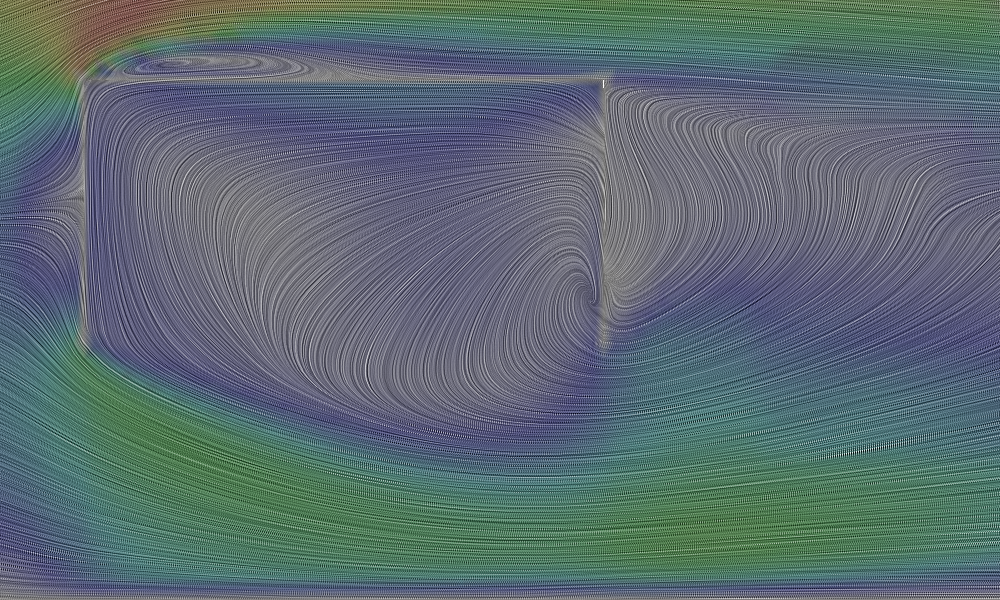
\includegraphics[height=4cm]{images/validation/refinement/mod/case_ref}}
		\annotatedFigureBox{0.091,0.7783}{0.343,0.9683}{A}{0.091,0.80}%bl
	\end{annotatedFigure}
	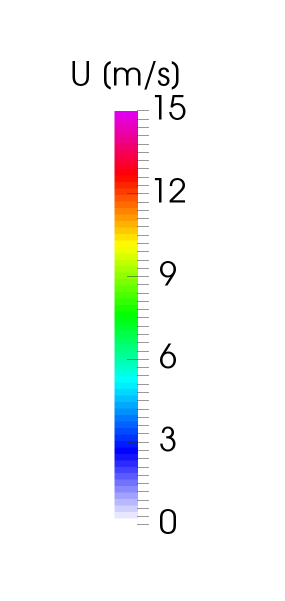
\includegraphics[width=0.15\linewidth]{images/validation/refinement/mod/scale_U}	
	\hfill
	\noindent\parbox[b][4cm][c]{2cm}{
		\subfloat[\mbox{normal}]{}
	} \vspace*{0.5cm}      \\  \hfill 
	\begin{annotatedFigure}
		{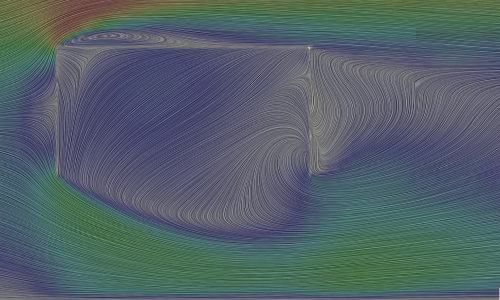
\includegraphics[height=4cm, trim= 2cm 0cm 0cm 0cm, clip]{images/validation/refinement/mod/case_fine}}
		\annotatedFigureBox{0.185,0.4634}{0.48,0.7416}{B}{0.185,0.4634}%bl
	\end{annotatedFigure}
	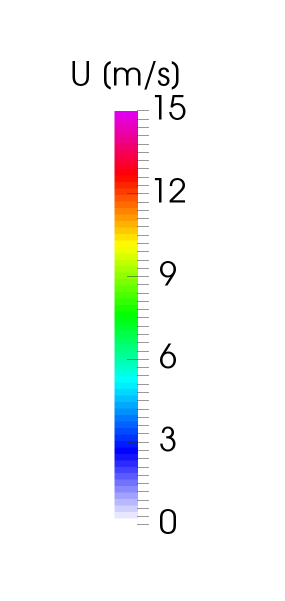
\includegraphics[width=0.15\linewidth]{images/validation/refinement/mod/scale_U}
	\hfill	
	\noindent\parbox[b][4cm][c]{2cm}{
		\subfloat[fine]{}
	}
	\begin{tikzpicture}[scale=1.5]
	\begin{scope}[overlay]
	\draw [->] (-9,1) -- (-8.7,1) node [below] {$y$};
	\draw [->] (-9,1) -- (-9,1.3) node [left] {$z$};
	\end{scope}			
	\end{tikzpicture}
	\captionsetup{format=plain}
	\caption[Flow pattern visualized by the LIC filter for all 4 stages of refinement]{Flow pattern visualized by the LIC filter for all 4 stages of refinement. Depicted is a vertical section through building of validation study. The flow direction is set in the positive y-direction. Both the normal and the find grid are able to resolve the standing vortex just above the geometry (\textbf{A}). The flow pattern in the geometry differs significantly for the fine mesh (\textbf{B}).}
	\label{fig:validation:grid_sens_LIC}
\end{figure}








\clearpage
\chapter{Tables}
\label{app:tables}
\renewcommand{\arraystretch}{1.2} %More linespacing for tables

\clearpage

	\begin{table}[h]
	\caption{Table with footnotes on the same page.}
	\begin{center}
		\begin{threeparttable}
			\begin{tabular}{c c c c}
				\toprule
				\textbf{1st Column} & \textbf{2nd Colimn} & \textbf{3rd Colimn} & \textbf{4th Colimn} \\ \midrule
				QWERTY\tnote{1}   &                     &                     &  \\
				ASDFGH\tnote{2}   &                     &                     &  \\ \bottomrule
			\end{tabular}
			\begin{tablenotes}
				\item[1] qwerty; \item[2] asdfgh
			\end{tablenotes}
		\end{threeparttable}
	\end{center}
	\label{table:simDisimCoefNewDef}
\end{table}

\clearpage


\input{tables/aerodynamic_roughness_length.tex}

}

%% Index
\printindex

\include{declaration}

% Cover on correct page
\clearpage
\thispagestyle{empty}
\vspace*{\fill}
\vspace*{\fill}
\clearpage
\includepdf[pages=1,trim=10cm 1.3cm 28cm 1.2cm,,fitpaper=false, pagecommand*={\thispagestyle{empty}}]{cover/cover.pdf}
\end{document}